% Created 2017-07-24 lun 09:35
% Intended LaTeX compiler: pdflatex
\documentclass[11pt]{article}
\usepackage[utf8]{inputenc}
\usepackage[T1]{fontenc}
\usepackage{graphicx}
\usepackage{grffile}
\usepackage{longtable}
\usepackage{wrapfig}
\usepackage{rotating}
\usepackage[normalem]{ulem}
\usepackage{amsmath}
\usepackage{textcomp}
\usepackage{amssymb}
\usepackage{capt-of}
\usepackage{hyperref}
\usepackage{minted}
\addtolength{\textwidth}{2in}
\addtolength{\hoffset}{-1in}
\addtolength{\voffset}{-1in}
\author{Patricio Martínez}
\date{\today}
\title{Introducción a JQuery}
\hypersetup{
 pdfauthor={Patricio Martínez},
 pdftitle={Introducción a JQuery},
 pdfkeywords={},
 pdfsubject={},
 pdfcreator={Emacs 26.0.50 (Org mode 9.0.9)}, 
 pdflang={English}}
\begin{document}

\maketitle
\tableofcontents


\section*{Introducción}
\label{sec:org8a2f91e}

Jquery es una librería que nos facilita muchas tareas comunes para nuestra web. Además nos ahorrará gran cantidad de tiempo y esfuerzo ya que nos permite crear muchos efectos y características con muy poco código.

\subsection*{Qué es JQuery}
\label{sec:orgc12639f}

JQuery es una rápida, liviana y con muchas características librería de JavaScript que se basa en el principio de \emph{escribir poco, y hacer mucho}. Permite hacer muchas tareas en nuestro documento sobre manipulación, manejar eventos, añadir animaciones y efectos de manera muy fácil

\subsection*{Ventajas de JQuery}
\label{sec:org62c0047}

Aquí algunas ventajas que tiene el adoptar JQuery:

\begin{itemize}
\item \textbf{Salva mucho tiempo} -- Te permite salvar mucho tiempo y esfuerzo al usar los selectores y animaciones de JQuery y así te puedes concentrar en el desarrollo.
\item Simplifica tareas comunes de JavaScript -- JQuery simplifica considerablemente las tareas más comunes de JavaScript. Podemos crear páginas ricas e interactivas con muy pocas líneas de código.
\item Fácil de usar - JQuery es muy fácil de usar. Cualquier persona con unos pocos conocimientos de HTML, CSS y JavaScript puede empezar a desarrollar con JQuery
\item Compatible con los navegadores -- JQuery es compatible con la mayoría de los navegadores modernos
\item Absolutamente gratis -- Es completamente libre para descargarlo y usarlo
\end{itemize}

\section*{Empezando con JQuery}
\label{sec:orgeb0da4c}

Para empezar con JQuery vamos a descararnos una copia e incluirla en nuestro documento. Podemos descararnos dos versiones, una comprimida y otra sin 
descomprimir. 

Una vez descargada la añadimos a nuestro documento en la cabecera tal como ya hemos visto. 

\subsection*{Incluyendo JQuery desde CDN}
\label{sec:orgbca6cf5}

Alternativamente, podemos incluir JQuery en tu página a través de un enlace a CDN (Content Delivery Network), si no queremos descargarlo. CDN nos ofrece la ventaja de reducir los tiempos de carga, ya que ellos tienen hospedaje en multitud de servidores a través de la tierra. Para enlazar JQuery directamente desde CDN añadimos el siguiente código:

\begin{minted}[]{html}
<script src="https://code.jquery.com/jquery-3.2.1.min.js"></script>
\end{minted}

\subsection*{Nuestra primera página con JQuery}
\label{sec:orgcad907d}

En esta página vamos a crear un Hola Mundo y le vamos a cambiar el color de la cabecera:

\begin{minted}[]{html}
<!DOCTYPE html>
<html>
<head>
    <meta charset="utf-8">
    <title>Nuestra primer página con JQuery</title>
    <link rel="stylesheet" type="text/css" href="css/style.css">
    <script src="js/jquery-3.2.1.min.js"></script>
    <script type="text/javascript">
        $(document).ready(function(){
            $("h1").css("color", "#0088ff");
        });
    </script>
</head>
<body>
    <h1>Hola, Mundo!</h1>
</body>
</html>
\end{minted}

\section*{Sintaxis de JQuery}
\label{sec:orgaf50fdc}

La sintaxis típica en JQuery empieza con el signo de dolar y termina con el punto y coma. 

Veamos el siguiente código:

\begin{minted}[]{html}
<script type="text/javascript">
$(document).ready(function(){
// algun código que ejecutar...
alert("Hola Mundo!");
});
</script>
</head>
<body>
<--! El contenido va aquí -->
</body>
</html>
\end{minted}

\subsection*{Explicación del código}
\label{sec:org7fa2caf}

Veamos las siguientes partes del código una por una:

\begin{itemize}
\item El elemento <script> -- Como JQuery es una librería, la llamamos desde un archivo externo
\item El \$(document)ready(manejador); -- Esto es típicamente conocido como un evento preparado. Básicamente es una función que le pasa al método ready() para ser ejecutado tan pronto como el documento empieza a ser manipulado
\end{itemize}

El método ready() es típicamente usado como una función anónima. 

Además dentro de la función nosotros escribimos la declaración JQuery que será la que hará la acción con la siguiente sintaxis: \$(selector).acción().

Donde, \$(selección) básicamente selecciona los elementos en el árbol de nodos DOM que puede ser manipulado y acción() aplica algunas acciones a los elementos seleccionados como cambiarle las propiedades CSS, cambiar el contenido, etc. 

Veamos el siguiente ejemplo:

\begin{minted}[]{html}
<!DOCTYPE html>
<html>
<head>
    <meta charset="utf-8">
    <title>Documento JQuery</title>
    <link rel="stylesheet" type="text/css" href="css/style.css">
    <script src="js/jquery-1.11.3.min.js"></script>
    <script type="text/javascript">
        $(document).ready(function(){
            $("p").text("Hola Mundo!");
        });
    </script>
</head>
<body>
    <p>No cargado todavía.</p>
</body>
</html>
\end{minted}

Aquí lo que vemos que hemos seleccionado el elemento <p> y con la acción \textbf{text} añadimos ese texto. 

Como vemos text reemplaza el texto. Veamos ahora el siguiente ejemplo:

\begin{minted}[]{html}
<!DOCTYPE html>
<html>
<head>
    <meta charset="utf-8">
    <title>Demo con JQuery</title>
    <link rel="stylesheet" type="text/css" href="/examples/css/style.css">
    <script src="https://code.jquery.com/jquery-1.12.4.min.js"></script>
    <script type="text/javascript">
        $(document).ready(function(){
            $("button").click(function(){
                $("p").text("Hola Mundo!");
            });            
        });
    </script>
</head>
<body>
    <p>No saludo al mundo.</p>
    <button type="button">Botón que reemplaza</button>
</body>
</html>  
\end{minted}

Ahora vemos como buscamos el elemento button y la acción se ejecuta con el pulsado del botón y lo que hace es a su vez buscar el elemento <p> y sustituir el texto. 


\section*{Seleccionando elementos con JQuery}
\label{sec:org1c68db2}

JavaScript es comúnmente usado para obtener o modificar contenido o atributos de los elementos HTML o aplicarles algunos efectos, animaciones, etc. 
Seleccionando elementos a través de JavaScript puede ser doloroso pero con JQuery todo resulta más fácil. La habilidad de hacer de forma simple selecciones de elementos del DOM es una de las características más potentes de JQuery. 

\subsection*{Seleccionando elementos por el ID}
\label{sec:org649c28c}

Ejemplo:

\begin{minted}[]{html}
<!DOCTYPE html>
<html>
<head>
<meta charset="utf-8">
<title>Seleccionando por ID en JQuery</title>
<script src="https://code.jquery.com/jquery-1.12.4.min.js"></script>
<script type="text/javascript">
$(document).ready(function(){
    // Cambia el color del elemento con id marca
    $("#marca").css("background", "yellow");
});
</script> 
</head>
<body>
    <p id="marca">Esto es un párrafo.</p>
    <p>Esto es otro párrafo.</p>
    <p>Y otro más.</p>
    <p><strong>Nota:</strong> El valor del id debe ser único.</p>
</body>
</html>                                		
\end{minted}

\subsection*{Seleccionando elementos por la clase}
\label{sec:orgf601f9e}

\begin{minted}[]{html}
<!DOCTYPE html>
<html>
<head>
<meta charset="utf-8">
<title>Seleccionando por ID en JQuery</title>
<script src="https://code.jquery.com/jquery-3.2.1.min.js"></script>
<script type="text/javascript">
$(document).ready(function(){

    $(".marca").css("background", "yellow");
});
</script> 
</head>
<body>
    <p class="marca">Esto es un párrafo.</p>
    <p class="marca">Esto es otro párrafo.</p>
    <p>Y otro más.</p>
</body>
</html>                                		
\end{minted}

\subsection*{Seleccionando por nombre}
\label{sec:org0def737}

\begin{minted}[]{html}
<!DOCTYPE html>
<html>
<head>
<meta charset="utf-8">
<title>Seleccionando por ID en JQuery</title>
<script src="https://code.jquery.com/jquery-3.2.1.min.js"></script>
<script type="text/javascript">
$(document).ready(function(){
    // Highlight element with id mark
    $("p").css("background", "yellow");
});
</script> 
</head>
<body>
    <p>Esto es un párrafo.</p>
    <p>Esto es otro párrafo.</p>
    <div>Y otro más.</div>
 </body>
</html>                                		
\end{minted}

\subsection*{Seleccionando por atributos}
\label{sec:org7f28126}

Con la palabra reservada \textbf{type} podemos elegir el tipo de atributo por el que queremos seleccionar el elemento.


\begin{minted}[]{html}
<!DOCTYPE html>
<html>
<head>
<meta charset="utf-8">
<title>Seleccionando elementos por atributos</title>
<script src="https://code.jquery.com/jquery-3.2.1.min.js"></script>
<script type="text/javascript">
$(document).ready(function(){

    $('input[type="text"]').css("background", "yellow");
});
</script>
</head>
<body>
    <form>
        <label>Nombre: <input type="text"></label>
        <label>Contraseña: <input type="password"></label>
        <input type="submit" value="Entra">
    </form>
</body>
</html>       
\end{minted}

\subsection*{Seleccionando elementos usando selectores de CSS compuestos}
\label{sec:orgde16cbe}

Podemos seleccionar selectores de CSS para hacer nuestra selección más precisa.

\begin{minted}[]{html}
<!DOCTYPE html>
<html>
<head>
<meta charset="utf-8">
<title>Seleccionando elementos por el selector</title>
<script src="https://code.jquery.com/jquery-3.2.1.min.js"></script>
<script type="text/javascript">
$(document).ready(function(){
    // Combinadmos el elemento párrafo con la clase marca
    $("p.mark").css("background", "yellow");

    // Combinamos span con el id marca
    $("#mark span").css("background", "yellow");

    // Combinamos dos elementos ul e il
    $("ul li").css("background", "yellow");

    // Combinamos dos elementos y el id marca
    $("ul#mark li").css("background", "red");

    // Combinamos dos marcas y la clase marca
    $("ul.mark li").css("background", "green");

    // Highlight all anchor elements with target blank
    $('a[target="_blank"]').css("background", "yellow");
});
</script>
</head>
<body>
    <p>Esto es un párrafo.</p>
    <p>Esto es otro párrafo.</p>
    <p>Otro más.</p>
    <ul>
        <li>Item uno</li>
        <li>Item dos</li>
        <li>Item tres</li>
    </ul>
    <ul id="marca">
        <li>Lista uno</li>
        <li>Lista dos</li>
        <li>Lista tres</li>
    </ul>
    <ul class="marca">
        <li>Y otro</li>
        <li>Pozi</li>
        <li>Pono</li>
    </ul>
    <p>Go to <a href="#">Inicio</a></p>
</body>
</html>                                		
\end{minted}

\subsection*{Selectores propios de JQuery}
\label{sec:org8704df3}

\begin{minted}[]{html}

<!DOCTYPE html>
<html>
<head>
<meta charset="utf-8">
<title>Selectores propios de JQuery</title>
<style type="text/css">
    /* Añadiendo estilo */
    *{
        padding: 5px;
    }
</style>
<script src="https://code.jquery.com/jquery-3.2.1.min.js"></script>
<script type="text/javascript">
$(document).ready(function(){
    // Selecciona las filas pares
    $("tr:odd").css("background", "yellow");

    // Selecciona las filas impares
    $("tr:even").css("background", "orange");

    // Selecciona el primer párrafo de un elemento
    $("p:first").css("background", "red");

    // Selecciona el último párrafo de un elemento
    $("p:last").css("background", "green");

    // Selecciona todo lo tipo text dentro de un formulario
    $("form :text").css("background", "purple");

    // Selecciona todo lo tipo password de un formulario
    $("form :password").css("background", "blue");

    // Selecciona todo los input de un formulario
    $("form :submit").css("background", "violet");
});
</script>
</head>
<body>
    <table border="1">
        <thead>
            <tr>
                <th>No.</th>
                <th>Nombre</th>
                <th>Email</th>
            </tr>
        </thead>
        <tbody>
            <tr>
                <td>1</td>
                <td>Paquito Chocolatero</td>
                <td>paco_elsobrao@mail.com</td>
            </tr>
            <tr>
                <td>2</td>
                <td>Juan Pérez</td>
                <td>juansinmiedo@mail.com</td>
            </tr>
            <tr>
                <td>3</td>
                <td>John Rambo</td>
                <td>johnrambo@mail.com</td>
            </tr>
        </tbody>
    </table>
    <p>Esto es un párrafo.</p>
    <p>Esto es otro.</p>
    <p>Que cansinos que sois.</p>
    <form>
        <label>Nombre: <input type="text"></label>
        <label>Contraseña: <input type="password"></label>
        <input type="submit" value="Sign In">
    </form>
</body>
</html>                                		
\end{minted}

\section*{Eventos en JQuery}
\label{sec:orgf0e5cd6}

Los eventos son interacciones del usuario con la página web. JQuery nos ofrece una gran cantidad de métodos para la mayoría de los eventos. Algunos de esos eventos son:

\begin{itemize}
\item ready()
\item click()
\item keypress()
\item focus()
\item blur()
\item change()
\item etc
\end{itemize}

Por ejemplo, el método ready() ejecuta algún código cuando el DOM está preparado.

\begin{minted}[]{html}
<!DOCTYPE html>
<html>
<head>
<meta charset="utf-8">
<title></title>
<script src="https://code.jquery.com/jquery-3.2.1.min.js"></script>
<script type="text/javascript">
$(document).ready(function(){
    alert("Hola Mundo!");
});
</script> 
</head>
<body>
    El contenido vendrá aquí
</body>
</html>         
\end{minted}

\subsection*{Eventos de ratón}
\label{sec:orge460457}

\subsubsection*{Método click()}
\label{sec:orgc79a88c}

El método *click() de JQuery une una función manejadora de eventos al elemento seleccionado por un evento "click". La función es ejectuado cuando el usuario pulsa el elemento. En el siguiente ejemplo esconderemos un elemento <p> de una página cuando son pulsado.

\begin{minted}[]{html}
<!DOCTYPE html>
<html>
<head>
<meta charset="utf-8">
<title>Ejecutando una función pulsando un elemento</title>
<script src="https://code.jquery.com/jquery-3.2.1.min.js"></script>
<style type="text/css">
    p{
        padding: 20px;
        font: 20px sans-serif;
        background: khaki;
    }
</style>
<script type="text/javascript">
$(document).ready(function(){
    $("p").click(function(){
        $(this).slideUp();
    });
});
</script>
</head>
<body>
    <p>Pínchame y desapareceré.</p>
    <p>Pínchame y desapareceré.</p>
    <p>Pínchame y desapareceré.</p>
</body>
</html>                                		
\end{minted}

\subsubsection*{El método dblclick()}
\label{sec:org22059be}

Este método es igual que el anterior solo que necesita que el usuario haga una doble pulsación sobre el elemento. Veámoslo en el ejemplo:


\begin{minted}[]{html}
<!DOCTYPE html>
<html>
<head>
<meta charset="utf-8">
<title>Ejecutando una función pulsando un elemento</title>
<script src="https://code.jquery.com/jquery-3.2.1.min.js"></script>
<style type="text/css">
    p{
        padding: 20px;
        font: 20px sans-serif;
        background: khaki;
    }
</style>
<script type="text/javascript">
$(document).ready(function(){
    $("p").dblclick(function(){
        $(this).slideUp();
    });
});
</script>
</head>
<body>
    <p>Pínchame y desapareceré.</p>
    <p>Pínchame y desapareceré.</p>
    <p>Pínchame y desapareceré.</p>
</body>
</html>
\end{minted}

\subsubsection*{El método hover()}
\label{sec:org98b4e7d}

El método hover() de JQuery une uno o dos funciones manejadoras de eventos a elementos seleccionados que se ejecutan cuando el puntero del ratón entra y deja los elementos. La primera función es ejecutada cuando el usuario pone el puntero en el elemento y la segunda es cuando el puntero deja el elemento. 

En este ejemplo se iluminará el elemento <p> cuando pongas el cursor sobre él y dejará de hacerlo cuando quites el puntero de él.

\begin{minted}[]{html}

<!DOCTYPE html>
<html>
<head>
<meta charset="utf-8">
<title>Ejecutando una función con el método hover()</title>
<script src="https://code.jquery.com/jquery-3.2.1.min.js"></script>
<style type="text/css">
    p{
        padding: 20px;
        font: 20px sans-serif;
        background: #f2f2f2;
    }
    p.highlight{
        background: red;
    }
</style>
<script type="text/javascript">
$(document).ready(function(){
    $("p").hover(function(){
        $(this).addClass("highlight");
    }, function(){
        $(this).removeClass("highlight");
    });
});
</script>
</head>
<body>
    <p>Tócame y me pongo rojito.</p>
    <p>Tócame y me pongo rojito.</p>
    <p>Tócame y me pongo rojito.</p>


</body>
</html>                                		
\end{minted}

\subsubsection*{El método mouseenter()}
\label{sec:org58fb42a}

Cómo sutilmente dice su propio nombre este método ejecuta la función cuando el puntero entra en el elemento. En el siguiente ejemplo el elemento se iluminará cuando el puntero se pose sobre él. 

\begin{minted}[]{html}
<!DOCTYPE html>
<html>
<head>
<meta charset="utf-8">
<title>Ejecutando una función con el método mouseenter()</title>
<script src="https://code.jquery.com/jquery-3.2.1.min.js"></script>
<style type="text/css">
    p{
        padding: 20px;
        font: 20px sans-serif;
        background: #f2f2f2;
    }
    p.highlight{
        background: red;
    }
</style>
<script type="text/javascript">
$(document).ready(function(){
    $("p").mouseenter(function(){
        $(this).addClass("highlight");
    });
    $("p").mouseleave(function(){
        $(this).removeClass("highlight");
    });
});
</script>
</head>
<body>

    <p>Tócame papi.</p>
    <p>Tócame papi.</p>
    <p>Tócame papi.</p>
</body>
</html>                                		
\end{minted}

\subsubsection*{El método mouseleave()}
\label{sec:orgcb41839}

Adivínalo tú solo que seguro que los sabes guapi.


\subsection*{Eventos del teclado}
\label{sec:orgf23ebc6}

\subsubsection*{El método keypress()}
\label{sec:org920986f}

Este método activa la une la función manejadora al elemento seleccionado (normalmente formularios) cuando el navegador recibe entrada del teclado por parte del usuario. El siguiente ejemplo se muestra un mensaje cuando el teclado es pulsado y además cuenta cuantas veces es pulsado el teclado:

\begin{minted}[]{html}
<!DOCTYPE html>
<html>
<head>
<meta charset="utf-8">
<title>Ejecutando una función con el evento Keypress</title>
<script src="https://code.jquery.com/jquery-1.12.4.min.js"></script>
<style type="text/css">
    p{
        padding: 10px;
        background: lightgreen;
        display: none;
    }
    div{
        margin: 20px 0;
    }
</style>
<script type="text/javascript">
$(document).ready(function(){
    var i = 0;
    $('input[type="text"]').keypress(function(){
        $("span").text(i += 1);
        $("p").show().fadeOut();
    });
});
</script>
</head>
<body>
    <input type="text">
    <div>Teclas Pulsadas: <span>0</span></div>
  <div><strong>Aviso:</strong> Escribe algo dentro de la caja, anda que te va a gustar....</div>
    <p>DAISYYYYY DAISYYYYY.</p>
</body>
</html>                                		
\end{minted}


\subsubsection*{El método keydown()}
\label{sec:orgf4a7741}

Es muy parecida al anterior pero la anterior ejecuta la función cuando la tecla es presionada y en esta es cuando la tecla es hundida

\subsubsection*{El método keyup()}
\label{sec:org1f82b65}

Pues más de lo mismo sólo que ahora la ejecución de la función es cuando la tecla es "soltada"


\subsection*{Eventos de formulario}
\label{sec:org3d74d29}

Los eventos de formularios se activan cuando cuando un control del formulario recibe o pierde el foco o cuando el usuario modifica un valor del formulario como cuando escribe en una caja de entrada, selecciona una selección de un caja de selección, etc. Vamos a ver algunos comunes.

\subsubsection*{El método change()}
\label{sec:orgcb615e3}

El método change() une una función manejadora a un elemento <input>, <textarea> y <select> que es ejecutado cuando el valor es cambiado. En el siguiente ejemplo se mostrará un mensaje de alerta cuando una opción en la caja de selección

\begin{minted}[]{html}
<!DOCTYPE html>
<html>
<head>
<meta charset="utf-8">
<title>Ejecutando una función cuando cambia un evento</title>
<script src="https://code.jquery.com/jquery-1.12.4.min.js"></script>
<script type="text/javascript">
$(document).ready(function(){
    $("select").change(function(){
        var selectedOption = $(this).find(":selected").val();
        alert("Te vas de vacaciones a - " + selectedOption);
    });
});
</script>
</head>
<body>
<h2>¿A qué ciudad vas a ir estas vaciones?</h2>
    <form>
        <label>Ciudad:</label>
        <select>
            <option>Roma</option>
            <option>Paris</option>
            <option>New York</option>
        </select>
    </form>
  <p><strong>Aviso:</strong> Selecciona un valor del menú desplegable.</p>
</body>
</html>                                		
\end{minted}

\subsubsection*{El método focus()}
\label{sec:orgccf2599}

Este método activa una función cuando seleccionamos elementos y gana el foco. En el siguiente ejemplo veremos un mensaje cuando la caja de entrada tenga foco.

\begin{minted}[]{html}
<!DOCTYPE html>
<html lang="en">
<head>
<meta charset="utf-8">
<title>Ejecutando una función cuando un evento tiene foco</title>
<script src="https://code.jquery.com/jquery-1.12.4.min.js"></script>
<style type="text/css">
    label{
        display: block;
        margin: 5px 0;
    }
    label span{
        display: none;
    }
</style>
<script type="text/javascript">
$(document).ready(function(){
    $("input").focus(function(){
        $(this).next("span").show().fadeOut("slow");
    });
});
</script>
</head>
<body>
    <form>
        <label>Email: <input type="text"> <span>Fíjate que no te vea nadie</span></label>
        <label>Contraseña: <input type="password"> <span>Cuida tus espaldas</span></label>
        <label><input type="submit" value="Entrar"> <span>Accede ahora</span></label>
    </form>
    <p><strong>Aviso:</strong> Con el ratón o con la tecla "TAB" tendrás foco.</p>
</body>
</html>                                		
\end{minted}

\subsubsection*{Método blur()}
\label{sec:orgc69fe48}

Ejecuta funciones cuando elementos tales como <input>, <textarea> o <select> pierden el foco.

\subsubsection*{Método submit()}
\label{sec:orgb95650c}
Este es para formularios, elementos <form> que ejecutan una función cuando el usuario envía un formulario. En el siguiente ejemplo se mostrará un mensaje cuando se vaya a enviar el mensaje.


\begin{minted}[]{html}
<!DOCTYPE html>
<html>
<head>
<meta charset="utf-8">
<title>Ejecuta una función cuando en un formulario se envía éste</title>
<script src="https://code.jquery.com/jquery-1.12.4.min.js"></script>
<style type="text/css">
    .error{
        color: red;
    }
    .success{
        color: green;
    }
</style>
<script type="text/javascript">
$(document).ready(function(){
    $("form").submit(function(event){
      var mob = /^[1-9]{1}[0-9]{9}$/;
        var currentValue = $("#inputMobile").val();
        if(mob.test(currentValue) == false && currentValue != 10){
            $("p").html("Número de teléfono inválido number").addClass("error").show().fadeOut(1000);
        } else{
            $("p").html("Número de teléfono válido number").addClass("success").show().fadeOut(1000);
        }
        event.preventDefault();
    });
});
</script>
</head>
<body>
    <form>
        <input type="text" id="inputMobile" maxlength="10" placeholder="Introduce un númemro de teléfono">
        <input type="submit" value="Submit">
        <p></p>
    </form>
</body>
</html>                                		
\end{minted}

\subsection*{Eventos en el documento/ventana}
\label{sec:org0984e3a}

Aquí los eventos son lanzados cuando un DOM está preparado o cuando la ventana se redimensiona o hay un scrol. Vamos a ver los más usados

\subsubsection*{El método ready()}
\label{sec:org71b48e2}

Éste ejecuta una función cuando el DOM está completamente cargado. En el siguiente ejemplo se reemplazará un texto cuando el DOM esté cargado.

\begin{minted}[]{html}
<!DOCTYPE html>
<html>
<head>
<meta charset="utf-8">
<title>Ejecutando una función con el método ready()</title>
<script src="https://code.jquery.com/jquery-1.12.4.min.js"></script>
<script type="text/javascript">
$(document).ready(function(){
    $("p").text("El DOM está cargado y preparado para ser manipulado.");
});
</script>
</head>
<body>
    <p>Espera un poquito.</p>
</body>
</html>                                		
\end{minted}

\subsubsection*{El método resize()}
\label{sec:orgf6a4c8b}

Este método activa una función cuando la ventana del navegador cambia de tamaño.

\begin{minted}[]{html}
<!DOCTYPE html>
<html>
<head>
<meta charset="utf-8">
<title>Ejecutando una función cuando redimensionamos la ventana</title>
<script src="https://code.jquery.com/jquery-1.12.4.min.js"></script>
<style type="text/css">
    p{
        padding: 20px;
        font: 20px sans-serif;
        background: #f0e68c;
    }
</style>
<script type="text/javascript">
$(document).ready(function(){
    $(window).resize(function() {
        $(window).bind("redimensiona", function(){ 
            $("p").text("Altura de la ventana: " + $(window).width() + ", " + "Altura de la ventana: " + $(window).height());
        });
    });
});
</script>
</head> 
<body>
    <p>Cambia el tamaño de la ventana</p>
</body>
</html>     
\end{minted}

\subsubsection*{Método scroll()}
\label{sec:orgbfc0422}

Esto activa la función cuadno detecta que el scroll de un iframe o de la ventana cambia. En este ejemplo se mostrará un mensaje cuadno el scroll del navegador cambia.

\begin{minted}[]{html}
<!DOCTYPE html>
<html>
<head>
<meta charset="utf-8">
<title>Ejecutando una función cuando hacemos scroll</title>
<script src="https://code.jquery.com/jquery-1.12.4.min.js"></script>
<style type="text/css">
    p{
        width: 100%;
        padding: 50px 0;
        text-align: center;
        font: bold 34px sans-serif;
        background: #f0e68c;
        position: fixed;
        top: 50px;
        display: none;
    }
    .dummy-content{
        height: 600px;
        font: 34px sans-serif;
        text-align: center;
    }
</style>
<script type="text/javascript">
$(document).ready(function(){
    $(window).scroll(function() {
        $("p").show().fadeOut("slow");
    });
});
</script> 
</head> 
<body>
    <p>Vamos que nos vamos!</p>
    <div class="dummy-content">Volando voy...</div>
    <div class="dummy-content">Volando vengo...</div>
    <div class="dummy-content">Por el camino...</div>
    <div class="dummy-content">Yo me entretengooo.</div>
    <div class="dummy-content">salalaaaaa.</div>
</body>
</html>                                		
\end{minted}

\section*{Efectos en JQuery}
\label{sec:orgc805f9e}

\subsection*{Efecto de mostrar y ocultar}
\label{sec:org3b1d80b}

Usando los métodos de JQuery \textbf{show()} y \textbf{hide()} podemos ocultar y mostrar elementos HTML.

El método hide() lo que hace simplemente es añadir en el estilo la propiedad \textbf{display:none} para ocultar el elemento. Por el contrario, el método show() lo que hace es restaurar la propiedad display a como estaba.

En este ejemplo podemos ver como funciona:

\begin{minted}[]{html}
<!DOCTYPE html>
<html>
<head>
<meta charset="UTF-8">
<title>Ejemplo del efecto de ocultar de JQuery</title>
<script src="https://code.jquery.com/jquery-1.12.4.min.js"></script>
<style type="text/css">
    p{
        padding: 15px;
        background: #F0E68C;
    }
</style>
<script type="text/javascript">
$(document).ready(function(){
    // Escondemos el párrafo
    $(".hide-btn").click(function(){
        $("p").hide();
    });

    // Mostramos el párrafo
    $(".show-btn").click(function(){
        $("p").show();
    });
});
</script>
</head>
<body>
    <button type="button" class="hide-btn">Esconde la tontá</button> 
    <button type="button" class="show-btn">Muestra la tontá</button>
    <p>Suavementeeee.</p>
    <p>Ocultameeeee.</p>
</body>
</html>                                		
\end{minted}

También podemos especificar la velocidad a la que queremos que se produzca este efecto. Para ello usaremos o bien las palabras predefinidas \textbf{'slow'} y \textbf{'fast'} o también podemos indicarlo con exactitud indicando los milisegundos. En el siguiente ejemplo vemos esto:

\begin{minted}[]{html}
<!DOCTYPE html>
<html>
<head>
<meta charset="UTF-8">
<title>Ejemplo de un efecto de mostrar/ocultar animado a distintas velocidades</title>
<script src="https://code.jquery.com/jquery-1.12.4.min.js"></script>
<style type="text/css">
    p{
        padding: 15px;
        background: #F0E68C;
    }
</style>
<script type="text/javascript">
$(document).ready(function(){
    // Escondemos los párrafos con distintas velocidades
    $(".hide-btn").click(function(){
        $("p.normal").hide();
        $("p.fast").hide("fast");
        $("p.slow").hide("slow");
        $("p.very-fast").hide(50);
        $("p.very-slow").hide(2000);
    });
 $(".show-btn").click(function(){
        $("p.normal").show();
        $("p.fast").show("fast");
        $("p.slow").show("slow");
        $("p.very-fast").show(50);
        $("p.very-slow").show(2000);
    });
});
</script>
</head>
<body>
    <button type="button" class="hide-btn">Esconde los párrafos</button> 
    <button type="button" class="show-btn">Muestra los párrafos</button>
    <p class="very-fast">Este párrafo se mostrará/ocultará muy rápido.</p>
    <p class="normal">Este párrafo se mostrará/ocultará con velocidad por defecto.</p>
    <p class="fast">Este párrafo se mostrará/ocultará de forma rápida.</p>
    <p class="slow">Este párrafo se mostrará/ocultará de forma lenta.</p>
    <p class="very-slow">Este párrafo se mostrará/ocultará de forma muy lenta.</p>
</body>
</html>                                		

\end{minted}

Al mismo tiempo que ocultamos/mostramos un elemento podemos hacer una llamada a otra función. Veamos este ejemplo que muestra una alerta cuando ocultamos o mostramos un párrafo.

\begin{minted}[]{html}
<!DOCTYPE html>
<html>
<head>
<meta charset="UTF-8">
<title>Ejemplo de llamada a otra función mietras mostramos/ocultamos</title>
<script src="https://code.jquery.com/jquery-1.12.4.min.js"></script>
<style type="text/css">
    p{
        padding: 15px;
        background: #F0E68C;
    }
</style>
<script type="text/javascript">
$(document).ready(function(){
    // Muestra un mensaje de alerta depués de esconder un párrafo
    $(".hide-btn").click(function(){
        $("p").hide("slow", function(){

            alert("El efecto de ocultación ha terminado.");
        });
    });

    // Muestra un mensaje de alerta depués de mostrar un párrafo
    $(".show-btn").click(function(){
        $("p").show("slow", function(){
           alert("El efecto de mostrado ha terminado.");
        });
    });
});
</script>
</head>
<body>
    <button type="button" class="hide-btn">Esconde el párrafo</button> 
    <button type="button" class="show-btn">Muestra el párrafo</button>
    <p>Esto es un párrafo.</p>
</body>
</html>                                		
\end{minted}

\subsubsection*{Efecto toggle()}
\label{sec:orgcee44fb}

Funciona exactamente igual que los métodos show() y hide(), solo que cambia el estado de oculto a mostrado y de mostrado a oculto.

\subsection*{Efecto fade}
\label{sec:org49c492e}

\subsubsection*{Métodos fadeIn() y fadeOut()}
\label{sec:org3243877}

En JQuery tenemos los métodos \textbf{fadeIn()} y \textbf{fadeOut()} para mostrar o esconder elementos pero de una incrementando o decrementando su opacidad.

Ejemplo:

\begin{minted}[]{html}
<!DOCTYPE html>
<html>
<head>
<meta charset="UTF-8">
<title>Ejemplos del efecto Fade-In y Fade-Out</title>
<script src="https://code.jquery.com/jquery-1.12.4.min.js"></script>
<style type="text/css">
    p{
        padding: 15px;
        background: #DDA0DD;
    }
</style>
<script type="text/javascript">
$(document).ready(function(){
    // Mostrando el párrafo
    $(".out-btn").click(function(){
        $("p").fadeOut();
    });

    // Ocultando el párrafo
    $(".in-btn").click(function(){
        $("p").fadeIn();
    });
});
</script>
</head>
<body>
    <button type="button" class="out-btn">largando párrafo</button>
    <button type="button" class="in-btn">trayendo párrafo</button>
    <p>Esto amigos es una cosa rosa.</p>
    <p>Yo soy otra cosa rosa.</p>
</body>
</html>                                		                                		
\end{minted}

Al igual que con el método anterior también podemos \textbf{controlar la velocidad} de igual manera y también podemos \textbf{hacer llamadas} a otras funciones

\subsubsection*{Método fadeToggle()}
\label{sec:org84eb7e6}

Exactamente igual que el anterior pero solo que si el elemento está presente lo oculta y si está oculto lo muestra.

\subsubsection*{Método fadeTo()}
\label{sec:org1a31301}

Este método es similar a fadeIn(), pero a diferencia de él fadeTo() nos permite controlar el nivel de opacidad. 

\begin{minted}[]{js}
$(selector).fadeTo(<velocidad>, <opacidad>, <llamada a otra función>);
\end{minted}

El parámetro de la opacidad es necesario y va entre 0  y 1 y también es requerida la velocidad de la animación.

Ejemplo:

\begin{minted}[]{html}
<!DOCTYPE html>
<html>
<head>
<meta charset="UTF-8">
<title>Ejemplo del efecto fade con FadeTo()</title>
<script src="https://code.jquery.com/jquery-1.12.4.min.js"></script>
<style type="text/css">
    p{
        display: none;
        padding: 15px;
        background: #DDA0DD;
    }
</style>
<script type="text/javascript">
$(document).ready(function(){
    // Fade con diferentes opacidades
    $(".to-btn").click(function(){
        $("p.none").fadeTo("fast", 0);
        $("p.partial").fadeTo("slow", 0.5);
        $("p.complete").fadeTo(2000, 1);
    });
});
</script>
</head>
<body>
    <button type="button" class="to-btn">Fade para esconder los distintos párrafos</button>
    <p class="none">Esto es un párrafo.</p>
    <p class="partial">Esto es otro párrafo.</p>
    <p class="complete">Y párrafo.</p>
</body>
</html>                                		                                		
\end{minted}

\subsection*{Efecto Sliding (corredero)}
\label{sec:org0b375a0}

\subsubsection*{Método slideUp() y slideDown()}
\label{sec:org2477643}

Los métodos slideUp() y slideDown() sirve para mostrar o esconder un elemento por incremento o decremento de su altura. 

Ejemplo:

\begin{minted}[]{html}
<!DOCTYPE html>
<html>
<head>
<meta charset="UTF-8">
<title>Ejemplo de los métodos slideUp() y slideDown()</title>
<script src="https://code.jquery.com/jquery-1.12.4.min.js"></script>
<style type="text/css">
    p{
        padding: 15px;
        background: #B0C4DE;
    }
</style>
<script type="text/javascript">
$(document).ready(function(){
    // Efecto de hacia arriba
    $(".up-btn").click(function(){
        $("p").slideUp();
    });

    // Efecto de hacia abajo
    $(".down-btn").click(function(){
        $("p").slideDown();
    });
});
</script>
</head>
<body>
    <button type="button" class="up-btn">Tira parriba</button> 
    <button type="button" class="down-btn">Tira pabajo</button>
    <p>Esto es un párrafo.</p>
    <p>Esto es otro párrafo.</p>
</body>
</html>                                		
\end{minted}

Al igual que los otros métodos vistos hasta ahora podemos controlar la velocidad y hacer llamadas a otras funciones en el proceso.

\subsubsection*{Método slideToggle()}
\label{sec:orgfe36ea8}

Muestra o oculta un elemento seleccionado con una animación que cambia su altura. En este método también podemos  controlar la velocidad y hacer llamadas a otras funciones.

\subsection*{Efectos de animación}
\label{sec:org114cfdb}

\subsubsection*{Método animate()}
\label{sec:org2e49227}

En JQuery el método animate() es usado para crear animaciones. Es usado con propiedades numéricas de CSS como son la altura, anchura, margen, relleno, opacidad, etc. Propiedades no numéricas como pueden ser el color no pueden ser animadas. Para animar color usamos un plugin especial llamado \href{https://github.com/jquery/jquery-color}{jquery-color}.

\subsubsection*{Sintaxis}
\label{sec:org2cfa061}

La sintaxis básica de animate() es:

\begin{minted}[]{js}
$(selector).animate({propiedades}, duración, llamada);
\end{minted}

Los parámetros de animate() tiene el siguiente significado:

\begin{itemize}
\item El parámetro propiedad es requerido y define la propiedad CSS que queremos animar.
\item La duración es opcional y la podemos especificar con las palabras \textbf{'slow'} y \textbf{'fast'} o poniendo un número que son los milisegundos.
\item La llamada a otra función es opcional
\end{itemize}

Veamos un ejemplo donde una imagen es animada y va desde una posición inicial hacia la derecha 300 píxeles.

\begin{minted}[]{html}
<!DOCTYPE html>
<html>
<head>
<meta charset="UTF-8">
<title>Ejemplo de efectos de animación</title>
<script src="https://code.jquery.com/jquery-1.12.4.min.js"></script>
<style type="text/css">
    img{
        position: relative; /* esto es requerido */
    }
</style>
<script type="text/javascript">
$(document).ready(function(){
    $("button").click(function(){
        $("img").animate({
            left: 300
        });
    });
});
</script>
</head>
<body>
    <button type="button">Empieza la animación</button>
    <p>
      <img src="/img/champi.jpg" alt="Toad">
    </p>
</body>
</html>                                		
\end{minted}

\subsubsection*{Animando múltiples propiedades a la vez}
\label{sec:org6e73c75}

Con el método animate() podemos animar varias propiedades a la vez.

Ejemplo:

\begin{minted}[]{html}
<!DOCTYPE html>
<html>
<head>
<meta charset="UTF-8">
<title>Ejemplo de una animación de múltiples propiedades</title>
<script src="https://code.jquery.com/jquery-1.12.4.min.js"></script>
<style type="text/css">
    .box{
        width: 100px;
        height: 100px;
        background: #9d7ede;
        margin-top: 30px;
        border-style: solid; /* Este valor es requerido */
        border-color: #6f40ce;
    }
</style>
<script type="text/javascript">
$(document).ready(function(){
    $("button").click(function(){
        $(".box").animate({
            width: "300px",
            height: "300px",
            marginLeft: "150px",
            borderWidth: "10px",
            opacity: 0.5
        });
    });
});
</script>
</head>
<body>
    <button type="button">Empieza la animación</button>
    <div class="box"></div>
</body>
</html>                                		
\end{minted}

\subsubsection*{Animando múltiples propiedades una a una o en fila.}
\label{sec:org6914f1c}

Podemos animar múltiples propiedades una a una de forma individual usando una característica de encadenamiento de JQuery. Lo veremos en el siguiente capítulo

\subsubsection*{Animando propiedades con valores relativos}
\label{sec:org313898f}

En ocasiones podemos usar valores relativos para animar propiedades. Si un valor es especificado con el prefijo \textbf{+=} o \textbf{-=} entonces se calcula el valor añadiendo o restando el valor dado al valor actual de la propiedad.

Ejemplo:

\begin{minted}[]{html}

<!DOCTYPE html>
<html>
<head>
<meta charset="UTF-8">
<title>Ejemplo de una animación con valores relativos</title>
<script src="https://code.jquery.com/jquery-1.12.4.min.js"></script>
<style type="text/css">
    .box{
        width: 100px;
        height: 100px;
        background: #9d7ede;
        margin-top: 30px;
        position: relative; /* Required to move element */
    }
</style>
<script type="text/javascript">
$(document).ready(function(){
    $("button").click(function(){
        $(".box").animate({            
            top: "+=50px",
            left: "+=50px",
            width: "+=50px",
            height: "+=50px"
        });
    });
});
</script>
</head>
<body>
    <button type="button">Empezar animación</button>
    <div class="box"></div>
</body>
</html>                                		

\end{minted}

\subsubsection*{Animando propiedades con valores Pre-definidos}
\label{sec:org0d580f0}

Además de los valores numéricos, cada propiedad puede tomar valores con las palabras \textbf{'show'}, \textbf{'hide'} y \textbf{'toggle'} 

Ejemplo:

\begin{minted}[]{html}
<!DOCTYPE html>
<html>
<head>
<meta charset="UTF-8">
<title>Ejemplo de una animación con los valores pre-definidos</title>
<script src="https://code.jquery.com/jquery-1.12.4.min.js"></script>
<style type="text/css">
    .box{
        width: 80%;
        height: 200px;
        background: #9d7ede;
        margin-top: 30px;
    }
</style>
<script type="text/javascript">
$(document).ready(function(){
    $("button").click(function(){
        $(".box").animate({
            width: 'toggle'
        });
    });
});
</script>
</head>
<body>
    <button type="button">Animación de cierre</button>
    <div class="box"></div>
</body>
</html>                                		
\end{minted}

\subsection*{Parada de las animaciones en JQuery}
\label{sec:org179b393}

\subsubsection*{El método stop()}
\label{sec:orgfdc52c0}

El método stop() es usado para parar las animaciones o efectos que estén funcionando. La sintaxis básica es:

\begin{minted}[]{js}
$(selector).stop(stopAll, goToEnd);
\end{minted}

Vamos a explicar los parámetros:

\begin{itemize}
\item El booleano \emph{stopAll} es opcional y detiene todas las animaciones. Su valor por defecto es \textbf{false} lo que significa que parará la animación que estemos citando en concreto y dejará a las demás.
\item El booleano \emph{goToEnd} si especifica si queremos completar la animación de forma inmediata. El valor por defecto es \textbf{false}
\end{itemize}

Veamos un ejemplo que demuestra como funciona el método stop() 

\begin{minted}[]{html}
<!DOCTYPE html>
<html>
<head>
<meta charset="UTF-8">
<title>Ejemplo de parada de una animación con stop()</title>
<script src="https://code.jquery.com/jquery-1.12.4.min.js"></script>
<style type="text/css">
    img{
        position: relative; /* propiedad requerida */
    }
</style>
<script type="text/javascript">
$(document).ready(function(){
    // Empieza la animación
    $(".start-btn").click(function(){
      $("img").animate({left: "+=150px"}, 2000);
    });

    // Stop running animation
    $(".stop-btn").click(function(){
      $("img").stop();
    });

    // Start animation in the opposite direction
    $(".back-btn").click(function(){
      $("img").animate({left: "-=150px"}, 2000);
    });

    // Reset to default
    $(".reset-btn").click(function(){
      $("img").animate({left: "0"}, "fast");
    });
});
</script>
</head>
<body>
    <button type="button" class="start-btn">Empezar</button>
    <button type="button" class="stop-btn">Parar</button>
    <button type="button" class="back-btn">Atrás</button>
    <button type="button" class="reset-btn">Reset</button>
    <p>
      <img src="/examples/images/mushroom.jpg" alt="Mushroom">
    </p>
</body>
</html>                                		                                		
\end{minted}

\subsection*{Encadenamiento en JQuery}
\label{sec:org5d40a8a}

\subsubsection*{El método Chaining (encadenamiento)}
\label{sec:org16758f6}

JQuery ofrece una característica robusta que nos permite unir múltiples acciones para el mismo grupo de elementos, todo en una sola línea de código.

Esto es posible porque los métodos en JQuery devuelven los objetos que pueden ser usados para llamar a otros métodos. Veamos un ejemplo:

\begin{minted}[]{html}
<!DOCTYPE html>
<html>
<head>
<meta charset="utf-8">
<title>Ejemplo de un método de encadenamiento</title>
<script src="https://code.jquery.com/jquery-1.12.4.min.js"></script>
<style type="text/css">
/* Algunos estilos bonitos */
p {
    width: 200px;
  padding: 40px 0;
  font: bold 24px sans-serif;
  text-align: center;
    background: #aaccaa;
    border: 1px solid #63a063;
    box-sizing: border-box;
}
</style>
<script type="text/javascript">
$(document).ready(function(){
    $(".start").click(function(){
        $("p").animate({width: "100%"}).animate({fontSize: "46px"}).animate({borderWidth: 30});
    });
    $(".reset").click(function(){
        $("p").removeAttr("style");
    });
});  
</script>
</head>
<body>
    <p>Hola fondo norteee!</p>
    <button type="button" class="start">Empezar encadenamiento</button>
    <button type="button" class="reset">Reset</button>
</body>
</html>                                		
\end{minted}

Hemos escrito todo el encadenamiento en una sola línea:

\begin{minted}[]{js}
$("p").animate({width: "100%"}).animate({fontSize: "46px"}).animate({borderWidth: 30});
\end{minted}

Pero si esto es muy embarullado podemos hacerlo en varias líneas

\begin{minted}[]{js}
$("p")
           .animate({width: "100%"})
           .animate({fontSize: "46px"})
           .animate({borderWidth: 30});
\end{minted}

\section*{Manipulando elementos en JQuery}
\label{sec:orgb028c29}

\subsection*{Getters y Setter en JQuery}
\label{sec:org6aa4499}

\subsubsection*{Obtener o establecer contenido y valores en JQuery}
\label{sec:orgb9ad848}

Algunos métodos en JQuery pueden ser usados para asignar o leer algunos valores een una selección. Unos pocos de esos métodos son \textbf{text(), html(), attr()} y \textbf{val()} 

Cuando esos métodos son llamados sin argumentos, son referidos como \emph{getters}, porque ellos obtienen (get) o leen los valores de los elementos. Cuando esos métodos son llamados con valores como argumentos, se refiere a ellos como  setters porque establecer o asignan (set) ese valor.

\subsubsection*{Método text()}
\label{sec:orgfc64f97}

El método text() es usado para obtener la combinación de texto de los contenidos seleccionados y sus descendientes, o establecer contenido de texto a los elementos seleccionados.

\begin{itemize}
\item Obteniendo contenido de texto con el método text()
\label{sec:org172ccce}

Vamos a ver como obtenemos el contenido de texto de los párrafos y los mostramos en una carteles de alerta:

\begin{minted}[]{html}
<!DOCTYPE html>
<html>
<head>
<meta charset="UTF-8">
<title>Ejemplo cómo obtener texto con text()</title>
<script src="https://code.jquery.com/jquery-1.12.4.min.js"></script>
<script type="text/javascript">
$(document).ready(function(){
    $(".btn-one").click(function(){
        var str = $("p").text();
        alert(str);
    });
    $(".btn-two").click(function(){
       var str = $("p:first").text();
       alert(str);
    });
    $(".btn-three").click(function(){
       var str = $("p.extra").text();
       alert(str);
    });
});
</script>
</head>
<body>
    <button type="button" class="btn-one">Obteniendo el texto de todos los párrafos</button>
    <button type="button" class="btn-two">Obteniendo el texto del primer párrafo</button>
  <button type="button" class="btn-three">Obteniendo el texto del último párrafo</button>
    <p>Esto es un párrafo.</p>
    <p>Esto es otro párrafo.</p>
  <p class="extra">Y uno más.</p>
</body>
</html>                                		
\end{minted}

\item Estableciendo contenido de texto con el método text()
\label{sec:org4e4acd9}

En el siguiente ejemplo veremos como el método text() establece contenido en un párrafo:

\begin{minted}[]{html}
<!DOCTYPE html>
<html>
<head>
<meta charset="UTF-8">
<title>Establecer texto con el métodos text()</title>
<script src="https://code.jquery.com/jquery-1.12.4.min.js"></script>
<script type="text/javascript">
$(document).ready(function(){
    $(".btn-one").click(function(){
        $("p").text("Esto es un texto de prueba.");
    });
    $(".btn-two").click(function(){
        $("p:first").text("Esto es otro texto de prueba.");
    });
    $(".btn-three").click(function(){
        $("p.empty").text("Esto es otro texto de prueba.");
    });
});
</script>
</head>
<body>
    <button type="button" class="btn-one">Establece texto en todos los párrafos</button>
    <button type="button" class="btn-two">Establece texto en el primer párrafo</button>
    <button type="button" class="btn-three">Establece texto en el párrafo vacío</button>
    <p>Esto es un párrafo.</p>
    <p>Esto es otro párrafo.</p>
    <p class="empty"></p>
</body>
</html>                                		
\end{minted}
\end{itemize}

\subsubsection*{Método html()}
\label{sec:orga634e5f}

El método html() es usado para obtener o establecer congtenido HTML de los elementos.

\begin{itemize}
\item Obtener contenido HTML con el método html()
\label{sec:org3c36be2}

En el siguiente ejemplo se verá como obtener el contenido HTML de los párrafos así como el contenido de un elemento <div>

\begin{minted}[]{html}
<!DOCTYPE html>
<html>
<head>
<meta charset="UTF-8">
<title>Obteniendo contenido HTML de un elemento</title>
<script src="https://code.jquery.com/jquery-1.12.4.min.js"></script>
<script type="text/javascript">
$(document).ready(function(){
    $(".btn-one").click(function(){
        var str = $("p").html();
        alert(str);
    });
    $(".btn-two").click(function(){
        var str = $("#container").html();
        alert(str);
    });
});
</script>
</head>
<body>
    <button type="button" class="btn-one">Obtener el contenido HTML de un párrafo</button>
    <button type="button" class="btn-two">Obtener el contenido HTML del contenedor</button>
    <div id="container">
        <h1>Hola People!</h1>
        <p>Tengo un <b>pie</p> más grande que otro.</p>
    </div>
</body>
</html>                                		
\end{minted}

\item Estableciendo contenido HTML con el método html()
\label{sec:orgaa9d870}

Veremos en el siguiente ejemplo como establecemos contenido en el elemento <body>

\begin{minted}[]{html}
<!DOCTYPE html>
<html>
<head>
<meta charset="UTF-8">
<title>Estableciendo contenido</title>
<script src="https://code.jquery.com/jquery-1.12.4.min.js"></script>
<script type="text/javascript">
$(document).ready(function(){
    $("button").click(function(){
        $("body").html("<p>Estoy harto de saludar!</p>");
    });
});
</script>
</head>
<body>
    <button type="button">Escribe un saludo</button>
</body>
</html>                                		
\end{minted}
\end{itemize}

\subsubsection*{Método attr()}
\label{sec:org392a197}

Podemos usar el método attr() para obtener el valor de un atributo o establecerlo

\begin{itemize}
\item Obtener el valor de un atributo con el método attr()
\label{sec:org5db96ee}

En el siguiente ejemplo veremos como obtener el atributo <href> del hiper enlace (elemento <a>) así como el atributo <alt> de un elemento imagen (<img>)

\begin{minted}[]{html}
<!DOCTYPE html>
<html>
<head>
<meta charset="UTF-8">
<title>Obteniendo el valor de un atributo de un elemento</title>
<script src="https://code.jquery.com/jquery-1.12.4.min.js"></script>
<script type="text/javascript">
$(document).ready(function(){
    $(".btn-one").click(function(){
        var str = $("a").attr("href");
        alert(str);
    });
    $(".btn-two").click(function(){
        var str = $("img#sky").attr("alt");
        alert(str);
    });
});
</script>
</head>
<body>
    <button type="button" class="btn-one">Obtenemos la referencia del enlace</button>
    <button type="button" class="btn-two">Obtenemos el valor del atributo ALT</button>
    <p><a href="https://www.fsf.com/">Free Software Foundation</a></p>
    <img id="sky" src="/examples/images/sky.jpg" alt="Cielo nuboso">
</body>
</html>                                		
\end{minted}

\item Establecer el valor de un atributo con el método attr()
\label{sec:orgc73a873}

En el siguiente ejemplo veremos como establecer el atributo \textbf{checked} en una caja de comprobación.

\begin{minted}[]{html}
<!DOCTYPE html>
<html>
<head>
<meta charset="UTF-8">
<title>Estableciendo un atributo con attr()</title>
<script src="https://code.jquery.com/jquery-1.12.4.min.js"></script>
<script type="text/javascript">
$(document).ready(function(){
    $("button").click(function(){
        $('input[type="checkbox"]').attr("checked", "checked");
    });
});
</script>
</head>
<body>
    <p><label><input type="checkbox"></label>Acepto los términos y condiciones y dejo que me des por donde amargan los pepinos.</p>
    <button type="button">Comprueba</button>
</body>
</html>                                		
\end{minted}
\end{itemize}

\subsubsection*{El metodo val()}
\label{sec:orge4e0ac5}

Se utiliza el método val() para obtener o establecer los valores actuales de elementos de formularios HTML tales como <input><select> y <textarea>

\begin{itemize}
\item Obteniendo los valores de los campos de un formulario con el método val()
\label{sec:org93f77db}

Veamos el siguiente ejemplo:

\begin{minted}[]{html}
<!DOCTYPE html>
<html>
<head>
<meta charset="UTF-8">
<title>Obteniendo los valores de un formulario</title>
<script src="https://code.jquery.com/jquery-1.12.4.min.js"></script>
<script type="text/javascript">
$(document).ready(function(){
    $("button.get-name").click(function(){
        var name = $("#name").val();
        alert(name);
    });
    $("button.get-comment").click(function(){
        var comment = $("#comment").val();
        alert(comment);
    });
    $("button.get-city").click(function(){
        var city = $("#city").val();
        alert(city);
    });
});
</script>
</head>
<body>
    <form>
        <table>
            <tr>
                <td>Nombre:</td>
                <td>
                    <input type="text" id="name">
                </td>
            </tr>
            <tr>
                <td>Comentarios:</td>
                <td>
                    <textarea rows="4" cols="30" id="comment"></textarea>
                </td>
            </tr>
            <tr>
                <td>Ciudad:</td>
                <td>
                    <select id="city">
                        <option>London</option>
                        <option>Paris</option>
                        <option>New York</option>
                    </select>
                </td>
            </tr>
        </table>
    </form>
    <p><strong>AVISO:</strong> Rellena los siguientes campos.</p>
    <button type="button" class="get-name">Obtén nombre</button>
    <button type="button" class="get-comment">Obtén comentario</button>
    <button type="button" class="get-city">Obtén ciudad</button>
</body>
</html>                        
\end{minted}

\item Estableciendo los valores de los campos de un formulario con el método val()
\label{sec:org89799b6}

Veamos el siguiente ejemplo:

\begin{minted}[]{html}
<!DOCTYPE html>
<html>
<head>
<meta charset="UTF-8">
<title>Estableciendo los valores en un formulario</title>
<script src="https://code.jquery.com/jquery-1.12.4.min.js"></script>
<script type="text/javascript">
$(document).ready(function(){
    $("button").click(function(){
        var text = $(this).text();
        $('input[type="text"]').val(text);
    });
});
</script>
</head>
<body>
<h2>Cual es la misión de la NASA que más te gusta?</h2>
    <button type="button">Discovery</button>
    <button type="button">Atlantis</button>
    <button type="button">Endeavour</button>
<p><strong><Aviso:></Aviso:>> Pulsa en los botones de arriba.</p>
    <p>
        <input type="text">
    </p>
</body>
</html>                                		
\end{minted}
\end{itemize}

\subsection*{Insertar contenido con JQuery}
\label{sec:org18ecd45}

JQuery dispone de varios métodos como append(), prepend(), html(), text(), before(), after(), wrap(), etc, que permite insertar nuevo contenido en un elemento existente.

Como ya hemos visto los métodos html() y text(), discutiremos los restantes.

\subsubsection*{Método append()}
\label{sec:org9bc0bed}

Este método se usa para insertar contenido al final de los elementos seleccionados. En el siguiente ejemplo veremos como se agrega algo de HTML a todos los párrafos y además añadimos contenido al pulsar un botón

\begin{minted}[]{html}
<!DOCTYPE html>
<html lang="en">
<head>
<meta charset="UTF-8">
<title>Inserting HTML Contents At the End of the Elements in jQuery</title>
<script src="https://code.jquery.com/jquery-1.12.4.min.js"></script>
<script type="text/javascript">
$(document).ready(function(){
    // Append all paragraphs on document ready
    $("p").append(' <a href="#">quiere saber más?</a>');

    // Append a div container on button click
    $("button").click(function(){
       $("#container").append("Esto es un texto de prueba.");
    });
});
</script>
</head>
<body>
    <button type="button">Inserta Texto</button>
    <div id="container">
        <p>Lorem ipsum dolor sit amet, consectetur adipiscing elit. Nam eu sem tempor, varius quam at, luctus dui. Mauris magna metus, dapibus nec turpis vel, semper malesuada ante.</p>
        <p>Quis quam ut magna consequat faucibus. Pellentesque eget nisi a mi suscipit tincidunt. Ut tempus dictum risus. Pellentesque viverra sagittis quam at mattis. Suspendisse potenti.</p>
    </div>
</body>
</html>                                		
\end{minted}

\subsubsection*{Método prepend()}
\label{sec:org03af09e}

El método \textbf{prepend()} es usado para insertar contenido al principio de los elementos seleccionados.

En el siguiente ejemplo añadiremos contenido al final de los párrafos y cuando pulsemos un botón.

\begin{minted}[]{html}
<!DOCTYPE html>
<html>
<head>
<meta charset="UTF-8">
<title>Insertando contenido HTML al principio de los elementos seleccionados</title>
<script src="https://code.jquery.com/jquery-1.12.4.min.js"></script>
<script type="text/javascript">
$(document).ready(function(){
    // Prepend all paragraphs on document ready
    $("p").prepend("<strong>AVISO:</strong> ");

    // Prepend a div container on button click
    $("button").click(function(){
       $("#container").prepend("Esto es un texto de prueba.");
    });
});
</script>
</head>
<body>
    <button type="button">Inserta Texto</button>
    <div id="container">
        <p>Lorem ipsum dolor sit amet, consectetur adipiscing elit. Nam eu sem tempor, varius quam at, luctus dui. Mauris magna metus, dapibus nec turpis vel, semper malesuada ante.</p>
        <p>Quis quam ut magna consequat faucibus. Pellentesque eget nisi a mi suscipit tincidunt. Ut tempus dictum risus. Pellentesque viverra sagittis quam at mattis. Suspendisse potenti.</p>
    </div>
</body>
</html>                                		
\end{minted}

\subsubsection*{Insertando múltiples elementos con los métodos append() y prepend()}
\label{sec:org8bd7ed2}

Tanto append() como prepend() soportan múltiples argumentos como entrada. 

En el siguiente ejemplo insertaremos <h1>,<p> y <img> dentro de <body>.

\begin{minted}[]{html}
<!DOCTYPE html>
<html>
<head>
<meta charset="UTF-8">
<title>Insertar múltiples elementos con append() y prepend()</title>
<script src="https://code.jquery.com/jquery-1.12.4.min.js"></script>
<script type="text/javascript">
$(document).ready(function(){
    $("button").click(function(){
        var newHeading = "<h1>Nota importante:</h1>";
        var newParagraph = document.createElement("p");
    newParagraph.innerHTML = "<em>Lorem Ipsum is dummy text...</em>";
        var newImage = $('<img src="/images/smiley.png" alt="Symbol">');
        $("body").append(newHeading, newParagraph, newImage);
    });
});
</script>
</head>
<body>
    <button type="button">Inserta Contenido</button>
    <p>Lorem ipsum dolor sit amet, consectetur adipiscing elit. Nam eu sem tempor, varius quam at, luctus dui. Mauris magna metus, dapibus nec turpis vel, semper malesuada ante, metus ac nisl bibendum.</p>
</body>
</html>                                		
\end{minted}

\subsubsection*{Método before() y after()}
\label{sec:org9f1b375}

Con estos métodos introducimos contenido antes y después de los elementos seleccionados.

Veamos un ejemplo:

\begin{minted}[]{html}
<!DOCTYPE html>
<html>
<head>
<meta charset="UTF-8">
<title>Insertando contenido antes y después de un elemento</title>
<script src="https://code.jquery.com/jquery-1.12.4.min.js"></script>
<script type="text/javascript">
$(document).ready(function(){
    // Add content after a div container on document ready
    $("#container").after("<p>— The End —</p>");

    // Add content before a div container on document ready
    $("#container").before("<p>— Demo Text —</p>");

    // Add content after heading on button click
    $("button.insert-after").click(function(){
        $("h1").after('<img src="/examples/images/marker-right.gif" alt="Symbol">');
    });

    // Add content before heading on button click
    $("button.insert-before").click(function(){
        $("h1").before('<img src="/examples/images/marker-left.gif" alt="Symbol">');
    });
});
</script>
<style type="text/css">
    h1{
        display: inline-block; 
    }
    body{
        text-align: center;
    }
</style>
</head>
<body>
    <h1>Bienvenidos</h1>
    <hr>
    <button type="button" class="insert-before">Inserta Antes</button>
    <button type="button" class="insert-after">Inserta Después</button>
    <hr>
    <div id="container">
        <p>Lorem ipsum dolor sit amet, consectetur adipiscing elit. Nam eu sem tempor, varius quam at, luctus dui. Mauris magna metus, dapibus nec turpis vel, semper malesuada ante. Vestibulum id metus ac nisl bibendum scelerisque non non purus. Suspendisse varius nibh non aliquet sagittis. In tincidunt orci sit amet elementum vestibulum. Vivamus fermentum in arcu in aliquam. Quisque aliquam porta odio in fringilla. Vivamus nisl leo, blandit at bibendum eu, tristique eget risus. Integer aliquet quam ut elit suscipit, id interdum neque porttitor. Integer faucibus ligula.</p>

    </div>
</body>
</html>   
\end{minted}

\subsubsection*{Método wrap()}
\label{sec:org70a2aa6}

El método wrap() es usado para envolver una estructura HTML alrededor de los elementos asociados. 

En el siguiente ejemplo envolveremos un div con una clase wrapper y un párrafo con un <em> y un <b>

\begin{minted}[]{html}
<!DOCTYPE html>
<html>
<head>
<meta charset="UTF-8">
<title>Ejemplo de envolver un elemento</title>
<script src="https://code.jquery.com/jquery-1.12.4.min.js"></script>
<script type="text/javascript">
$(document).ready(function(){
    // Envolviendo un div con otro div
    $(".container").wrap('<div class="wrapper"></div>');

    // Envolviendo un párrafo al pulsar un botón
    $("button").click(function(){
        $("p").contents().wrap("<em><b></b></em>");
    });
});
</script>
<style type="text/css">
    .wrapper{
        padding: 20px;
        background: #f0e68c;
        margin: 10px 0;
    }
    .container{
        padding: 15px;
        background: #fff;
        font-size: 24px;
    }
</style>
</head>
<body>
    <button type="button">Púlsame para envolver</button>
    <div class="container">
        <p>Esto es un texto de prueba.</p>
    </div>
</body>
</html>                                		
\end{minted}

\subsection*{Eliminar contenido con JQuery}
\label{sec:org6bd73c2}

JQuery tiene métodos muy útiles tales como empty(), remove(), unwrap(), etc para eliminar elementos o contenido HTML existentes del documento

\subsubsection*{Método empty()}
\label{sec:org0e8dea4}

Este método elimina todos los elementos hijo así como otros descendientes  el contenido de texto de un elemento seleccionado desde el DOM. 

En el siguiente ejemplo se elimina todo el contenido dentro de los elementos con la clase .container al pulsar un botón.

\begin{minted}[]{html}
<!DOCTYPE html>
<html>
<head>
<meta charset="utf-8">
<title>Eliminando contenido</title>
<style type="text/css">
.container{
    padding: 10px;
    background: #f0e68C;
    border: 1px solid #bead18;
}
</style>
<script src="https://code.jquery.com/jquery-1.12.4.min.js"></script>
<script type="text/javascript">
$(document).ready(function(){

    $("button").click(function(){
       $(".container").empty();
    });
});
</script>
</head>
<body>
    <div class="container">
        <h1>Buenos días por la mañana!</h1>
        <p class="hint"><strong>Aviso:</strong> Si pulsas el botón lo borrarás todo incluído el botón</p>
        <button type="button">Vaciar contenedor</button>
    </div>
</body>
</html>                                		
\end{minted}


\subsubsection*{El método remove()}
\label{sec:org81a8f5f}

Este método elimina los elementos seleccionados y todo lo que hay dentro de él.

En el siguiente ejemplo borraremos todos los elementos <p> con la clase .hint. Los elementos dentro de ese elemento también serán borrados

\begin{minted}[]{html}
<!DOCTYPE html>
<html>
<head>
<meta charset="utf-8">
<title>Eliminando elementos desde el DOM</title>
<style type="text/css">
.container{
    padding: 10px;
    background: #f0e68C;
    border: 1px solid #bead18;
}
</style>
<script src="https://code.jquery.com/jquery-1.12.4.min.js"></script>
<script type="text/javascript">
$(document).ready(function(){
    // Borra el párrafo con la clase hint
    $("button").click(function(){
       $("p.hint").remove();
    });
});
</script>
</head>
<body>
    <div class="container">
        <h1>Saluditos vecinitos!</h1>
        <p class="hint"><strong>Aviso:</strong> Si pulsas este botón borrarás el párrafo.</p>
        <button type="button">Borra el párrafo</button>
    </div>
</body>
</html>                                		
\end{minted}

\subsubsection*{El método unwrap()}
\label{sec:orge2b66d6}

Elimina todo lo que hay alrededor de un elmento. Hace lo contrario que el método wrap()

\subsubsection*{El método removeAttr()}
\label{sec:org2704849}

Elimina los atributos de un elemento selecciondo.

En el siguiente ejemplo borraremos el atributo href de un elemento <a> al pulsar un botón

\begin{minted}[]{html}
<!DOCTYPE html>
<html>
<head>
<meta charset="utf-8">
<title>Eliminando un atributo</title>
<style type="text/css">
  a{
        font-size: 18px;
    margin-right: 20px;
  }
</style>
<script src="https://code.jquery.com/jquery-1.12.4.min.js"></script>
<script type="text/javascript">
$(document).ready(function(){
    // Eliminamos el atributo href
    $("button").click(function(){
        $("a").removeAttr("href");
    });
});
</script>
</head>
<body>
    <div class="container">
        <p>
      <a href="">Inicio</a>
      <a href="">Sobre</a>
      <a href="">Contacto</a>
    </p>
        <button type="button">Borra atributos</button>
    </div>
</body>
</html>                                		
\end{minted}

\subsection*{Clases CSS con JQuery}
\label{sec:orgcbc54a7}

JQuery ofrece métodos para la manipulación de clases tales como addClass(), removeClass(), toggleClass, etc. 

\subsubsection*{Método addClass}
\label{sec:org553bbc9}

Este método añade una o más clases al elemento seleccionado 

Ejemplo:

\begin{minted}[]{html}
<!DOCTYPE html>
<html>
<head>
<meta charset="utf-8">
<title>Añadiendo clases a un elemento</title>
<style type="text/css">
    .page-header{
        color: red;
        text-transform: uppercase;
    }
    .highlight{
        background: yellow;
    }         
</style>
<script src="https://code.jquery.com/jquery-1.12.4.min.js"></script>
<script type="text/javascript">
$(document).ready(function(){
    $("button").click(function(){
        $("h1").addClass("page-header highlight");
    });
});
</script>
</head>
<body>
    <h1>Saluditos</h1>
    <p>Ganicas locas de que no haga tanto calor.</p>
    <button type="button">Añade clases</button>
</body>
</html>                                		
\end{minted}

\subsubsection*{Método removeClass()}
\label{sec:orgab8799a}

Elimina clases de los elementos seleccionados

Ejemplo:

\begin{minted}[]{html}
<!DOCTYPE html>
<html>
<head>
<meta charset="utf-8">
<title>Eliminando clases en JQuery</title>
<style type="text/css">
    .page-header{
        color: red;
        text-transform: uppercase;
    }
    .highlight{
        background: yellow;
    }        
</style>
<script src="https://code.jquery.com/jquery-1.12.4.min.js"></script>
<script type="text/javascript">
$(document).ready(function(){
    $("button").click(function(){
        $("h1").removeClass();
        $("p").removeClass();
    });
});
</script>
</head>
<body>
    <h1 class="page-header">Texto de prueba</h1>
    <p>Lorem ipsum dolor sit amet, consectetur adipiscing elit...</p>
    <p class="hint highlight"><strong>Nota:</strong> Lorem Ipsum is dummy text.</p>
    <button type="button">Eliminando clases</button>
</body>
</html>                                		
\end{minted}

\subsubsection*{Método toggleClass()}
\label{sec:org73b3e69}

Este método añade o borra según sea la selección clases de los elementos seleccionados

Ejemplo:

\begin{minted}[]{html}
<!DOCTYPE html>
<html>
<head>
<meta charset="utf-8">
<title>Cambiando clases con JQuery</title>
<style type="text/css">
    p{
        padding: 10px;
        cursor: pointer;        
        font: bold 16px sans-serif;
    }
    .highlight{
        background: yellow;
    }         
</style>
<script src="https://code.jquery.com/jquery-1.12.4.min.js"></script>
<script type="text/javascript">
$(document).ready(function(){
    $("p").click(function(){
        $(this).toggleClass("highlight");
    });
});
</script>
</head>
<body>
    <p>Pinchame y me pondré rojo o no.</p>
    <p class="highlight">Pinchame y me pondré rojo o no.</p>
    <p>Pinchame y me pondré rojo o no.</p>
</body>
</html>                                		
\end{minted}

\subsection*{Propiedades de estilo con JQuery}
\label{sec:org3b178a9}

JQuery también nos ofrece los métodos para obtener y establecer propiedadades CSS 

\subsubsection*{Método css()}
\label{sec:orgd0604af}

Este es un método rápido para acceder a los estilos de los elementos HTML

\begin{itemize}
\item Obtener el valor actual CSS
\label{sec:orgbf8d09a}

Podemos obtener el valor de la propiedad CSS de un elemento simplemente pasando el nombre de la propiedad como un parámetro al método css(). Aquí vemos la sintaxis básica:

\begin{minted}[]{js}
$(selector).css("nombrePropiedad");
\end{minted}

Ejemplo:

\begin{minted}[]{html}
<!DOCTYPE html>
<html>
<head>
<meta charset="utf-8">
<title>Obteniendo valores de una propiedad CSS</title>
<style type="text/css">
    div{
        width: 100px;
        height: 100px;
        margin: 10px;
        cursor: pointer;
        display: inline-block;
    }        
</style>
<script src="https://code.jquery.com/jquery-1.12.4.min.js"></script>
<script type="text/javascript">
$(document).ready(function(){
    $("div").click(function(){
        var color = $(this).css("background-color");
        $("#result").html(color);
    });    
});
</script>
</head>
<body>
    <div style="background-color:orange;"></div>
    <div style="background-color:#ee82ee;"></div>
    <div style="background-color:rgb(139,205,50);"></div>
    <div style="background-color:#f00;"></div>
    <p>El valor del color de fondo es: <b id="result"></b></p>
</body>
</html>                                		
\end{minted}

\item Establecer una propiedad CSS y su valores
\label{sec:org3432986}

El método css() pueden tomar el nombre de una propiedad y un valor como parámetros separados para establecerlos en una propiedad CSS para el elemento. Veamos el siguiente ejemplo:

\begin{minted}[]{html}

<!DOCTYPE html>
<html>
<head>
<meta charset="utf-8">
<title>Estableciendo valores de una propiedad CSS</title>
<style type="text/css">
    .box{
        width: 100px;
        height: 100px;
        margin: 10px;
        cursor: pointer;
        border: 1px solid #cdcdcd;
        display: inline-block;
    }        
</style>
<script src="https://code.jquery.com/jquery-1.12.4.min.js"></script>
<script type="text/javascript">
$(document).ready(function(){
    $(".box").click(function(){
        $(this).css("background-color", "red");
    });    
});
</script>
</head>
<body>
    <div class="box"></div>
    <div class="box"></div>
    <div class="box"></div>
    <div class="box"></div>
  <p><strong>Aviso:</strong> Pulsa dentro de la caja vacía para llenarla con el color de fondo.</p>
</body>
</html>
\end{minted}

\item Establecer múltiples propiedades CSS
\label{sec:org7af7704}

También podemos establecer múltiples valores CSS con el método css(). La sintaxis básica es:

\begin{minted}[]{js}
$(selector).css({"nombrePropiedad":"valor", "nombrePropiedad":"valor",...})
\end{minted}

Veamos el siguiente ejemplo:

\begin{minted}[]{html}
<!DOCTYPE html>
<html>
<head>
<meta charset="utf-8">
<title>Establecer el valor CSS de múltiples propiedades</title>
<style type="text/css">
    p{
        font-size: 18px;
        font-family: Arial, sans-serif;
    }
</style>
<script src="https://code.jquery.com/jquery-1.12.4.min.js"></script>
<script type="text/javascript">
$(document).ready(function(){
    $("button").click(function(){
        $("p").css({"background-color": "yellow", "padding": "20px"});
    });    
});
</script>
</head>
<body>
    <h1>Saludos desde la tierra</h1>
    <p style="background-color:orange;">Esto es un párrafo.</p>
    <p style="background-color:#ee82ee;">Esto es otro párrafo.</p>
    <p style="background-color:rgb(139,205,50);">Y otro más.</p>
    <p>El último párrafo.</p>
    <button type="button">Añadiendo estilo CSS</button>
</body>
</html>                                		
\end{minted}
\end{itemize}





\subsection*{Dimensiones en JQuery}
\label{sec:orgb76b183}

Vamos a aprender como obtener y establecer dimensiones en una caja tal como altura o anchura.

JQuery ofrece varios métodos, tales como height(), innerHeight(), outerHeight(), width(), innerWidth() y outerWidth() para obtener y establecer dimensiones CSS para los elementos. En la siguiente ilustración entenderemos como esos métodos calculan la s dimensiones de una caja.

\begin{center}
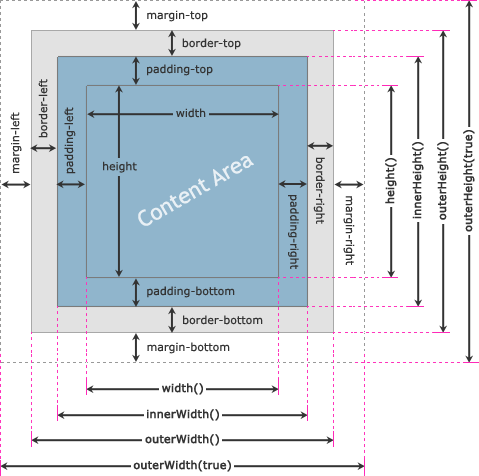
\includegraphics[width=.9\linewidth]{./img/dimensiones-jquery.png}
\end{center}



\subsubsection*{Métodos width() y height()}
\label{sec:org88fc940}

Los métodos width() y height() obtienen o establecer la \uline{altura} y la \uline{anchura} de los elementos. La altura y anchura no incluye relleno (padding), bode (border) y margen (margin) de el elemento. El siguiente ejemplo nos devolverá la altura y anchura de un elemento div

\begin{minted}[]{html}
<!DOCTYPE html>
<html>
<head>
<meta charset="utf-8">
<title>Obteniendo la altura y anchura de un elemento</title>
<style type="text/css">
    #box{
        width: 300px;
        height: 200px;
        padding: 25px;
        text-align: justify;
        border: 10px solid #c6b51a;
        background: #f0e68c;
        margin: 15px;
    }        
</style>
<script src="https://code.jquery.com/jquery-1.12.4.min.js"></script>
<script type="text/javascript">
$(document).ready(function(){
    $("button").click(function(){
        var divWidth = $("#box").width();
        var divHeight = $("#box").height();
        $("#result").html("Altura: " + divWidth + ", " + "Anchura: " + divHeight);
    });
});
</script>
</head>
<body>
    <div id="box">Lorem ipsum dolor sit amet, consectetur adipiscing elit. Nam eu sem tempor, varius quam at, luctus dui. Mauris magna metus, dapibus nec turpis vel, semper malesuada ante. Vestibulum id metus ac nisl bibendum scelerisque non non purus. Suspendisse varius nibh non aliquet sagittis. In tincidunt orci sit amet elementum vestibulum. Vivamus fermentum in arcu in aliquam. Quisque aliquam porta odio in fringilla non purus nisld Dapibus nec turpis vel, semper malesuada ant.</div>
    <button type="button">Obtén la altura y anchura</button>
    <p id="result"></p>
</body>
</html>                                		
\end{minted}

De manera similar podemos establecer al altura y anchura de los elementos incluyendo los parámetros en los métodos width() y height(). El valor puede ser una cadena de texto (número y unidad. ej: 100px, 20em) o un número. En el siguiente ejemplo estableceremos la altura de un elemennto <div> a 400 pixeles y una anchura de 300 píxeles respectivamente.

\begin{minted}[]{html}
<!DOCTYPE html>
<html>
<head>
<meta charset="utf-8">
<title>Estableciendo la altura y anchura de un elemento</title>
<style type="text/css">
    #box{
        width: 300px;
        height: 200px;
        padding: 25px;
        text-align: justify;
        border: 10px solid #c6b51a;
        background: #f0e68c;
        margin: 15px;
    }        
</style>
<script src="https://code.jquery.com/jquery-1.12.4.min.js"></script>
<script type="text/javascript">
$(document).ready(function(){
    $("button").click(function(){
        $("#box").width(400).height(300);
    });
});
</script>
</head>
<body>
    <div id="box">Lorem ipsum dolor sit amet, consectetur adipiscing elit. Nam eu sem tempor, varius quam at, luctus dui. Mauris magna metus, dapibus nec turpis vel, semper malesuada ante. Vestibulum id metus ac nisl bibendum scelerisque non non purus. Suspendisse varius nibh non aliquet sagittis. In tincidunt orci sit amet elementum vestibulum. Vivamus fermentum in arcu in aliquam. Quisque aliquam porta odio in fringilla non purus nisld Dapibus nec turpis vel, semper malesuada ant.</div>
    <button type="button">Establece al altura y la anchura</button>
</body>
</html>                                		
\end{minted}

\subsubsection*{Métodos innerWidth() y innerHeight()}
\label{sec:org1adcebd}

Los métodos de JQuery innerWidth() e innerHeight() obtienen o establecen el interior de la altura y la anchura de los elementos respectivamente. El interior incluye el relleno pero excluye el borde y el margen de los elementos. En el siguiente ejemplo obtendremos el valor de altura y anchura de un elemento <div>

\begin{minted}[]{html}
<!DOCTYPE html>
<html>
<head>
<meta charset="utf-8">
<title>Obteniendo la altura y anchura interiores</title>
<style type="text/css">
    #box{
        width: 300px;
        height: 200px;
        padding: 25px;
        text-align: justify;
        border: 10px solid #c6b51a;
        background: #f0e68c;
        margin: 15px;
    }        
</style>
<script src="https://code.jquery.com/jquery-1.12.4.min.js"></script>
<script type="text/javascript">
$(document).ready(function(){
    $("button").click(function(){
        var divWidth = $("#box").innerWidth();
        var divHeight = $("#box").innerHeight();
        $("#result").html("Inner Width: " + divWidth + ", " + "Inner Height: " + divHeight);
    });
});
</script>
</head>
<body>
    <div id="box">Lorem ipsum dolor sit amet, consectetur adipiscing elit. Nam eu sem tempor, varius quam at, luctus dui. Mauris magna metus, dapibus nec turpis vel, semper malesuada ante. Vestibulum id metus ac nisl bibendum scelerisque non non purus. Suspendisse varius nibh non aliquet sagittis. In tincidunt orci sit amet elementum vestibulum. Vivamus fermentum in arcu in aliquam. Quisque aliquam porta odio in fringilla non purus nisld Dapibus nec turpis vel, semper malesuada ant.</div>
    <button type="button">Obten la altura y anchura interior</button>
    <p id="result"></p>
  <hr>
  <p><strong>Aviso:</strong><b>innerWidth()</b> incluye las propiedades (<b>width</b> + <b>padding-left</b> + <b>padding-right</b>), e <b>innerHeight()</b> incluye (<b>height</b> + <b>padding-top</b> + <b>padding-bottom</b>).</p>
</body>
</html>                                		
\end{minted}

De igual manera, podemos establecer al altura y anchura interiores. Al alterar el innerWidth() y el innerHeight() también alteramos la altura y la anchura del área de contenido.

Por ejemplo, si la actual altura de un elemento es 300 píxeles y la suma de el relleno izquierdo y derecho es igual a píxeles entonces la nueva altura del elemento para obtener una altura de 4000 será de 350, es decir, \textbf{la nueva altura = altura interior - relleno horizontal}. Se puede estimar lo mismo con la altura.

\begin{minted}[]{html}
<!DOCTYPE html>
<html>
<head>
<meta charset="utf-8">
<title>Establecer alturas y anchuras interiores</title>
<style type="text/css">
    #box{
        width: 300px;
        height: 200px;
        padding: 25px;
        text-align: justify;
        border: 10px solid #c6b51a;
        background: #f0e68c;
        margin: 15px;
    }        
</style>
<script src="https://code.jquery.com/jquery-1.12.4.min.js"></script>
<script type="text/javascript">
$(document).ready(function(){
    $("button").click(function(){
        $("#box").innerWidth(400).innerHeight(300);
    });
});
</script>
</head>
<body>
    <div id="box">Lorem ipsum dolor sit amet, consectetur adipiscing elit. Nam eu sem tempor, varius quam at, luctus dui. Mauris magna metus, dapibus nec turpis vel, semper malesuada ante. Vestibulum id metus ac nisl bibendum scelerisque non non purus. Suspendisse varius nibh non aliquet sagittis. In tincidunt orci sit amet elementum vestibulum. Vivamus fermentum in arcu in aliquam. Quisque aliquam porta odio in fringilla non purus nisld Dapibus nec turpis vel, semper malesuada ant.</div>
    <button type="button">Establecer altura y anchura interiores</button>
</body>
</html>                                		

\end{minted}

\subsubsection*{Métodos outerWidth() y outerHeight()}
\label{sec:orga82500e}

Los métodos outerWidth() y outerHeight() sirven para establecer u obtener la altura y anchura exterior. Esto incluye el relleno y el borde pero excluye el margen del elemento. En el siguiente ejemplo devolverá la altura y anchura exteriores de un elemento <div>Y

\begin{minted}[]{html}
<!DOCTYPE html>
<html>
<head>
<meta charset="utf-8">
<title>Obteniendo la altura y anchura exteriores</title>
<style type="text/css">
    #box{
        width: 300px;
        height: 200px;
        padding: 25px;
        text-align: justify;
        border: 10px solid #c6b51a;
        background: #f0e68c;
        margin: 15px;
    }        
</style>
<script src="https://code.jquery.com/jquery-1.12.4.min.js"></script>
<script type="text/javascript">
$(document).ready(function(){
    $("button").click(function(){
        var divWidth = $("#box").outerWidth();
        var divHeight = $("#box").outerHeight();
        $("#result").html("Outer Width: " + divWidth + ", " + "Outer Height: " + divHeight);
    });
});
</script>
</head>
<body>
    <div id="box">Lorem ipsum dolor sit amet, consectetur adipiscing elit. Nam eu sem tempor, varius quam at, luctus dui. Mauris magna metus, dapibus nec turpis vel, semper malesuada ante. Vestibulum id metus ac nisl bibendum scelerisque non non purus. Suspendisse varius nibh non aliquet sagittis. In tincidunt orci sit amet elementum vestibulum. Vivamus fermentum in arcu in aliquam. Quisque aliquam porta odio in fringilla non purus nisld Dapibus nec turpis vel, semper malesuada ant.</div>
    <button type="button">Obtén la altura y anchura exteriores</button>
    <p id="result"></p>
  <hr>
  <p><strong>Aviso:</strong><b>outerWidth()</b> incluye las propiedades CSS (<b>width</b> + <b>padding-left</b> + <b>padding-right</b> + <b>border-left</b> + <b>border-right</b>), y el <b>outerHeight()</b> incluye (<b>height</b> + <b>padding-top</b> + <b>padding-bottom</b> + <b>border-top</b> + <b>border-bottom</b>).</p>
</body>
</html>                                		
\end{minted}

Podemos obtener también la altura y anchura incluyendo relleno y borde al igual que el margen del elemento. Para ello añadiremos el parámetro \textbf{true} al método tal como outerWidth(true) y outerHeight(true)

Ejemplo:

\begin{minted}[]{html}
<!DOCTYPE html>
<html>
<head>
<meta charset="utf-8">
<title>Obteniendo la altura y anchura con el margen</title>
<style type="text/css">
    #box{
        width: 300px;
        height: 200px;
        padding: 25px;
        text-align: justify;
        border: 10px solid #c6b51a;
        background: #f0e68c;
        margin: 15px;
    }        
</style>
<script src="https://code.jquery.com/jquery-1.12.4.min.js"></script>
<script type="text/javascript">
$(document).ready(function(){
    $("button").click(function(){
        var divWidth = $("#box").outerWidth(true);
        var divHeight = $("#box").outerHeight(true);
        $("#result").html("Outer Width: " + divWidth + ", " + "Outer Height: " + divHeight);
    });
});
</script>
</head>
<body>
    <div id="box">Lorem ipsum dolor sit amet, consectetur adipiscing elit. Nam eu sem tempor, varius quam at, luctus dui. Mauris magna metus, dapibus nec turpis vel, semper malesuada ante. Vestibulum id metus ac nisl bibendum scelerisque non non purus. Suspendisse varius nibh non aliquet sagittis. In tincidunt orci sit amet elementum vestibulum. Vivamus fermentum in arcu in aliquam. Quisque aliquam porta odio in fringilla non purus nisld Dapibus nec turpis vel, semper malesuada ant.</div>
    <button type="button">Obten la altura y anchura exteriores con el margen</button>
    <p id="result"></p>
  <hr>
  <p><strong>Note:</strong><b>outerWidth(true)</b> incluye (<b>width</b> + <b>padding-left</b> + <b>padding-right</b> + <b>border-left</b> + <b>border-right</b> + <b>margin-left</b> + <b>margin-right</b>), y <b>outerHeight(true)</b> incluye (<b>height</b> + <b>padding-top</b> + <b>padding-bottom</b> + <b>border-top</b> + <b>border-bottom</b> + <b>margin-top</b> + <b>margin-bottom</b>).</p>
</body>
</html>                                		
\end{minted}

De igual manera podemos establecer la altura y anchura exteriores añadiendo el valor como parámetro a los métodos. Ahora el calculo sería el siguiente para la anchura: 

\begin{itemize}
\item \textbf{Altura - (Relleno horizontal + borde horizontal)}
\end{itemize}

Ejemplo:

\begin{minted}[]{html}
<!DOCTYPE html>
<html lang="en">
<head>
<meta charset="utf-8">
<title>Estableciendo la altura y anchura exteriores</title>
<style type="text/css">
    #box{
        width: 300px;
        height: 200px;
        padding: 25px;
        text-align: justify;
        border: 10px solid #c6b51a;
        background: #f0e68c;
        margin: 15px;
    }        
</style>
<script src="https://code.jquery.com/jquery-1.12.4.min.js"></script>
<script type="text/javascript">
$(document).ready(function(){
    $("button").click(function(){
        $("#box").outerWidth(400).outerHeight(300);
    });
});
</script>
</head>
<body>
    <div id="box">Lorem ipsum dolor sit amet, consectetur adipiscing elit. Nam eu sem tempor, varius quam at, luctus dui. Mauris magna metus, dapibus nec turpis vel, semper malesuada ante. Vestibulum id metus ac nisl bibendum scelerisque non non purus. Suspendisse varius nibh non aliquet sagittis. In tincidunt orci sit amet elementum vestibulum. Vivamus fermentum in arcu in aliquam. Quisque aliquam porta odio in fringilla non purus nisld Dapibus nec turpis vel, semper malesuada ant.</div>
    <button type="button">Establece la altura y anchura exteriores</button>
</body>
</html>                                		
\end{minted}

\section*{JQuery avanzado}
\label{sec:orgedee325}

\subsection*{JQuery Traversing (recorrido)}
\label{sec:org1c10c6d}

\subsubsection*{Qué es el traversing}
\label{sec:org9a201a9}

Los selectores de JQuery nos permiten seleccionar los elementos recorriendo el árbol DOM. Pero en muchas ocasiones necesitamos seleccionar un elemento padre y uno antepasado. Ahí es donde entra en juego el método de recorrido por el DOM. Con esos método por demos ir hacia arriba, abajo y alrededor del árbol DOM muy fácilmente. 

El recorrido DOM es una muy prominente característica de JQuery. Para hacer esto necesitamos entender las relaciones entre los elementos de un árbol DOM. 

Ejemplo:

\begin{minted}[]{html}
<!DOCTYPE html>
<html>
<head>
<meta charset="utf-8">
<title>Ejemplo de árbol DOM</title>
<script src="https://code.jquery.com/jquery-1.12.4.min.js"></script>
</head>
<body>
    <div class="container">
        <h1>Hola Mundo</h1>
        <p>Esto es <em>un simple párrafo</em>.</p>
        <ul>
            <li>Item Uno</li>
            <li>Item Dos</li>
        </ul>
    </div>
</body>
</html>                                		
\end{minted}


El código HTML de este ejemplo lo podemos representar como este árbol DOM:


\begin{center}
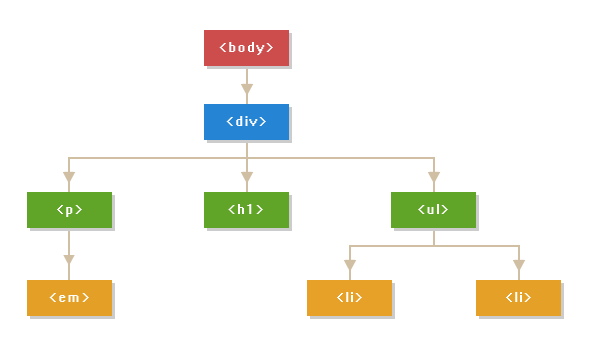
\includegraphics[width=.9\linewidth]{./img/arbol-dom.png}
\end{center}


El diagrama anterior muestra las relaciones padre/hijo entre los elementos:

\begin{itemize}
\item El elemento \emph{<body>} es \textbf{padre} del elemento \emph{<div>} y es el antepasado de todo. El elemento \emph{<div>} es \textbf{padre} de \emph{<h1>,<p>} y \emph{<ul>}, e \textbf{hijo} del elemento \emph{<body>}.
\item El elemento \emph{<h1>}, \emph{<p>} y \emph{<ul>} son \textbf{hermanos}, desde que tienen el mismo padre.
\item El elemento \emph{<h1>} es un \textbf{hijo} del elemento \emph{<div>} y un \textbf{descendiente} del elemento \emph{<body>}. Este elemento no tiene ningún hijo
\item El elemento \emph{<p>} es el padre del elemento \emph{<em>}, \textbf{hijo} del elemento \emph{<div>} y \textbf{descendiente} del elemento \emph{<body>}. El elemento \emph{<em>} es un \textbf{hijo} del elemento \emph{<p>} y un \textbf{descendiente} de los elementos \emph{<div>} y \emph{<body>}
\end{itemize}


\subsubsection*{Recorriendo el árbol DOM}
\label{sec:org867b334}

Ahora que hemos entendido las relaciones lógicas entre los elementos en un árbol DOM. En los siguiente capítulos aprenderemos como hacer operaciones para recorrer el árbol hacia arriba y hacia abajo usando JQuery

\subsection*{Antepasados}
\label{sec:org0b3b4f9}

\subsubsection*{Recorriendo el árbol DOM hacia arriba}
\label{sec:org4ba7d0f}

En las relaciones lógicas un antepasado es un padre, abuelo, bisabuelo y así.

JQuery dispone de métodos muy útiles tales como \textbf{parent(), parents() y parentsUntil()} que pueden usarse para recorrer el árbol DOM hacia arriba entre uno o múltiples niveles.

\subsubsection*{Método parent()}
\label{sec:org5eb3fd1}

El método \textbf{parent()} es usado para obtener directamente el padre del elemento seleccionado.

En el siguiente ejemplo resaltaremos el padre directo del elemento <li> es cual es <ul> añadiendo la clase .higlight

\begin{minted}[]{html}
<!DOCTYPE html>
<html>
<head>
<meta charset="utf-8">
<title>Seleccionando el padre de un elemento</title>
<script src="https://code.jquery.com/jquery-1.12.4.min.js"></script>
<script type="text/javascript">
$(document).ready(function(){
    $("li").parent().addClass("highlight");
});
</script>
</head>
<body>
    <div class="container">
        <h1>Hola Mundo</h1>
        <p>Esto es <em>un simple párrafo</em>.</p>
        <ul>
            <li>Item Uno</li>
            <li>Item Dos</li>
        </ul>
    </div>
</body>
</html>                                	
\end{minted}

\subsubsection*{El método parents()}
\label{sec:org450b1b8}

El método \textbf{parents()} es usado para obtener los antepasados de un elemento seleccionado. En el siguiente ejemplo añadiremos un borde alrededor de todos los elementos antepasados del elemento <li>, los cuales son <ul>, <div>, <body> y <html>

Ejemplo:

\begin{minted}[]{html}
<!DOCTYPE html>
<html>
<head>
<meta charset="utf-8">
<title>Seleccionando todos los antepasados de un elemento</title>
<style type="text/css">
    *{
        margin: 10px;
    }
    .frame{
        border: 2px solid green;
    }        
</style>
<script src="https://code.jquery.com/jquery-1.12.4.min.js"></script>
<script type="text/javascript">
$(document).ready(function(){
    $("li").parents().addClass("frame");
});
</script>
</head>
<body>
    <div class="container">
        <h1>Hola Mundo</h1>
        <p>Esto es <em>un simple párrafo</em>.</p>
        <ul>
            <li>Item Uno</li>
            <li>Item Dos</li>
        </ul>
    </div>
</body>
</html>                                		
\end{minted}

Podemos opcionalmente incluir uno o más selectores como parámetros en el método parents() para filtrar la búsqueda de los antepasados. En el siguiente ejemplo aplicaremos un borde al antepasado de <li> que son los elementos <div>.

\begin{minted}[]{html}
<!DOCTYPE html>
<html>
<head>
<meta charset="utf-8">
<title>Seleccionando un antepasado específico</title>
<style type="text/css">
    *{
        margin: 10px;
    }
    .frame{
        border: 2px solid green;
    }        
</style>
<script src="https://code.jquery.com/jquery-1.12.4.min.js"></script>
<script type="text/javascript">
$(document).ready(function(){
    $("li").parents("div").addClass("frame");
});
</script>
</head>
<body>
    <div class="container">
        <h1>Hola Mundo</h1>
        <p>Esto es<em>un simple párrafo</em>.</p>
        <ul>
            <li>Item Uno</li>
            <li>Item Dos</li>
        </ul>
    </div>
</body>
</html>                                		
\end{minted}

\subsubsection*{Método parentsUntil()}
\label{sec:orga6d2f4a}

Este método se usa para obtener todos los antepasados sin incluir el elemento que coincida con el selector. En palabras simples podemos pedir que nos devuelva todos los elementos antepasados entre dos elementos dados.

En el siguiente ejemplo vamos a añadir un bode alrededor de todos los elementos antepasados de <li> excluyendo <html>, es decir, añadiremos un borde a <ul>, <div> y <body>

\begin{minted}[]{html}
<!DOCTYPE html>
<html lang="en">
<head>
<meta charset="utf-8">
<title>Selecting All the Ancestors between Two Elements in jQuery</title>
<style type="text/css">
    *{
        margin: 10px;
    }
    .frame{
        border: 2px solid green;
    }        
</style>
<script src="https://code.jquery.com/jquery-1.12.4.min.js"></script>
<script type="text/javascript">
$(document).ready(function(){
    $("li").parentsUntil("html").addClass("frame");
});
</script>
</head>
<body>
    <div class="container">
        <h1>Hola Mundo</h1>
        <p>Esto es <em>un simple párrafo</em>.</p>
        <ul>
            <li>Item Uno</li>
            <li>Item Dos</li>
        </ul>
    </div>
</body>
</html>                                		
\end{minted}

\subsection*{Descendientes}
\label{sec:orga703229}

\subsubsection*{Recorriendo el árbol DOM hacia abajo}
\label{sec:orga89f13d}

En las relaciones lógicas un descendiente es un hijo, nieto, gran nieto, y así.

JQuery provee de métodos muy útiles tales como \textbf{children()} y \textbf{find()} que se pueden usar para recorrer hacia abajo por el árbol DOM uno o varios niveles de manera muy fácil y encontrar u obtener hijos u otros descendientes de un elemento en la jerarquía.

\subsubsection*{Método children()}
\label{sec:org78c2a58}

El método children() es usado para obtener directamente el hijo de un elemento. En el siguiente ejemplo resaltaremos el hijo directo del elemento <ul> el cual es <li> añadiendo la clase .highlight. 

\begin{minted}[]{html}
<!DOCTYPE html>
<html>
<head>
<meta charset="utf-8">
<title>Seleccionando hijos con JQuery</title>
<style type="text/css">
    .highlight{
        background: yellow;
    }        
</style>
<script src="https://code.jquery.com/jquery-1.12.4.min.js"></script>
<script type="text/javascript">
$(document).ready(function(){
    $("ul").children().addClass("highlight");
});
</script>
</head>
<body>
    <div class="container">
        <h1>Hola Mundo</h1>
        <p>Esto es <em>un simple párrafo</em>.</p>
        <ul>
            <li>Item Uno</li>
            <li>Item Dos</li>
        </ul>
    </div>
</body>
</html>                                		
\end{minted}

\subsubsection*{El método find()}
\label{sec:org0a3ea06}

El método find() es usado para obtener los descendientes de un elemento seleccionado. 

Los métodos find() y children() son similares, excepto que find() busca a través de múltiples niveles en el árbol hasta el último descendiente, mientras que children() solo lo hace un nivel. En el siguiente ejemplo añadiremos un borde alrededor de todos los elementos <li> que sean descendientes del elemento <div>.

\begin{minted}[]{html}
<!DOCTYPE html>
<html>
<head>
<meta charset="utf-8">
<title>Seleccionando hijos con JQuery</title>
<style type="text/css">
    .highlight{
        background: yellow;
    }        
</style>
<script src="https://code.jquery.com/jquery-1.12.4.min.js"></script>
<script type="text/javascript">
$(document).ready(function(){
    $("ul").find("li").addClass("frame");
});
</script>
</head>
<body>
    <div class="container">
        <h1>Hola Mundo</h1>
        <p>Esto es <em>un simple párrafo</em>.</p>
        <ul>
            <li>Item Uno</li>
            <li>Item Dos</li>
        </ul>
    </div>
</body>
</html>                                		
\end{minted}


Sin embargo, si queremos obtener todos los descendientes podemos usar el selector universal

\begin{minted}[]{html}
<!DOCTYPE html>
<html>
<head>
<meta charset="utf-8">
<title>Seleccionando hijos con JQuery</title>
<style type="text/css">
    .highlight{
        background: yellow;
    }        
</style>
<script src="https://code.jquery.com/jquery-1.12.4.min.js"></script>
<script type="text/javascript">
$(document).ready(function(){
    $("ul").find("*").addClass("frame");
});
</script>
</head>
<body>
    <div class="container">
        <h1>Hola Mundo</h1>
        <p>Esto es <em>un simple párrafo</em>.</p>
        <ul>
            <li>Item Uno</li>
            <li>Item Dos</li>
        </ul>
    </div>
</body>
</html>                                		
\end{minted}

\subsection*{Hermanos}
\label{sec:orga1b1f3e}

\subsubsection*{Recorriendo el árbol DOM lateralmente}
\label{sec:org66ec5fc}

En las relaciones lógicas los hermanos son los elementos que tienen el mismo padre.

JQuery provee de varios métodos tales como \textbf{siblings(), nest(), nestAll(), nextUntil(), prev(), prevAll() y prevUntil()} que podemos usar.

\subsubsection*{Método siblings()}
\label{sec:org580b690}

El método es usado para obtener el elemento hermano de un elemento seleccionado. En el siguiente ejemplo resaltaremos el hermano de <p> que son <h1> y <ul>.


\begin{minted}[]{html}
<!DOCTYPE html>
<html>
<head>
<meta charset="utf-8">
<title>Seleccionando hermanos con JQuery</title>
<style type="text/css">
    .highlight{
        background: yellow;
    }        
</style>
<script src="https://code.jquery.com/jquery-1.12.4.min.js"></script>
<script type="text/javascript">
$(document).ready(function(){
    $("p").siblings().addClass("highlight");
});
</script>
</head>
<body>
    <div class="container">
        <h1>Hola Mundo</h1>
        <p>Esto es <em>un simple párrafo</em>.</p>
        <ul>
            <li>Item Uno</li>
            <li>Item Dos</li>
        </ul>
    </div>
</body>
</html>                                		
\end{minted}

Opcionalmente podemos incluir uno o más selectores como parámetros en el metodo siblings() para filtrar nuestra búsqueda. En el siguiente ejemplo aplicaremos un borde alrededor de los hermanos de <p> que sea elementos <ul>.

\begin{minted}[]{html}
<!DOCTYPE html>
<html>
<head>
<meta charset="utf-8">
<title>Seleccionando hermanos específicos con JQuery</title>
<style type="text/css">
    .highlight{
        background: yellow;
    }        
</style>
<script src="https://code.jquery.com/jquery-1.12.4.min.js"></script>
<script type="text/javascript">
$(document).ready(function(){
    $("p").siblings("ul").addClass("highlight");
});
</script>
</head>
<body>
    <div class="container">
        <h1>Hola Mundo</h1>
        <p>Esto es <em>un simple párrafo</em>.</p>
        <ul>
            <li>Item Uno</li>
            <li>Item Dos</li>
        </ul>
    </div>
</body>
</html>                                		
\end{minted}

\subsubsection*{Método next()}
\label{sec:org05ac013}

El método next() es usado para para obtener el siguiente hermano del elemento seleccionado. En el siguiente ejemplo vamos a resaltar el próximo hermano de <p> que es <ul>.

\begin{minted}[]{html}
<!DOCTYPE html>
<html>
<head>
<meta charset="utf-8">
<title>Seleccionando el siguiente hermano con JQuery</title>
<style type="text/css">
    .highlight{
        background: yellow;
    }        
</style>
<script src="https://code.jquery.com/jquery-1.12.4.min.js"></script>
<script type="text/javascript">
$(document).ready(function(){
    $("p").next().addClass("highlight");
});
</script>
</head>
<body>
    <div class="container">
        <h1>Hola Mundo</h1>
        <p>Esto es <em>un simple párrafo</em>.</p>
        <ul>
            <li>Item Uno</li>
            <li>Item Dos</li>
        </ul>
    </div>
</body>
</html>                                		
\end{minted}

\subsubsection*{Método nextAll()}
\label{sec:org15a39a0}

Este método es usado para obtener todos los hermanos que siguen del elemento seleccionado. En el siguiente ejemplo resaltaremos todos los hermanos de <p>

\begin{minted}[]{html}
<!DOCTYPE html>
<html>
<head>
<meta charset="utf-8">
<title>Seleccionando hijos con JQuery</title>
<style type="text/css">
    .highlight{
        background: yellow;
    }        
</style>
<script src="https://code.jquery.com/jquery-1.12.4.min.js"></script>
<script type="text/javascript">
$(document).ready(function(){
    $("p").nextAll().addClass("highlight");
});
</script>
</head>
<body>
    <div class="container">
        <h1>Hola Mundo</h1>
        <p>Esto es <em>un simple párrafo</em>.</p>
        <ul>
            <li>Item Uno</li>
            <li>Item Dos</li>
        </ul>
    </div>
</body>
</html>                                		
\end{minted}

\subsubsection*{El método nextUntil()}
\label{sec:orgcfa8f9e}

Este método es usado para obtener todos los hermanos que sigan sin incluir el elemento que coincide con el selector. 

En el siguiente ejemplo resaltaremos los hermanos de <h1> excluyendo <ul>

\begin{minted}[]{html}
<!DOCTYPE html>
<html>
<head>
<meta charset="utf-8">
<title>Seleccionando todos los elementos hermanos entre dos elementos</title>
<style type="text/css">
    .highlight{
        background: yellow;
    }        
</style>
<script src="https://code.jquery.com/jquery-1.12.4.min.js"></script>
<script type="text/javascript">
$(document).ready(function(){
    $("h1").nextUntil("ul").addClass("highlight");
});
</script>
</head>
<body>
    <div class="container">
        <h1>Hola Mundo</h1>
        <p>Esto es <em>un simple párrafo</em>.</p>
        <ul>
            <li>Item Uno</li>
            <li>Item Dos</li>
        </ul>
    </div>
</body>
</html>                                		
\end{minted}

\subsubsection*{El método prev()}
\label{sec:org0916135}

Este método es usado para obtener el elemento hermano que inmediatamente precede. En el siguiente ejemplo resaltaremos  el hermano previo de <ul> el cual es el elemento <p>.

\begin{minted}[]{html}
<!DOCTYPE html>
<html>
<head>
<meta charset="utf-8">
<title>Seleccionando el hermano previo en JQuery</title>
<style type="text/css">
    .highlight{
        background: yellow;
    }        
</style>
<script src="https://code.jquery.com/jquery-1.12.4.min.js"></script>
<script type="text/javascript">
$(document).ready(function(){
    $("ul").prev().addClass("highlight");
});
</script>
</head>
<body>
    <div class="container">
        <h1>Hola Mundo</h1>
        <p>Esto es <em>un simple párrafo</em>.</p>
        <ul>
            <li>Item Uno</li>
            <li>Item Dos</li>
        </ul>
    </div>
</body>
</html>                                		
\end{minted}

\subsubsection*{El método prevAll()}
\label{sec:org2d69753}

Con el obtenemos todos los hermanos que preceden al elemento seleccionado. 

En el siguiente ejemplo resaltaremos a todos los hermanos que preceden a <ul>

\begin{minted}[]{html}
<!DOCTYPE html>
<html>
<head>
<meta charset="utf-8">
<title>Seleccionando a todos los hermanos con JQuery</title>
<style type="text/css">
    .highlight{
        background: yellow;
    }        
</style>
<script src="https://code.jquery.com/jquery-1.12.4.min.js"></script>
<script type="text/javascript">
$(document).ready(function(){
    $("ul").prevAll().addClass("highlight");
});
</script>
</head>
<body>
    <div class="container">
        <h1>Hola Mundo</h1>
        <p>Esto es <em>un simple párrafo</em>.</p>
        <ul>
            <li>Item Uno</li>
            <li>Item Dos</li>
        </ul>
    </div>
</body>
</html>                                		
\end{minted}

\subsubsection*{Método prevUntil()}
\label{sec:org6322a78}

Este método es usado para seleccionar a todos los hermanos previos hasta el que coincida con el selector. 

En el siguiente ejemplo vamos a resaltar todos los elementos hermanos previos de <ul> excluyendo al elemento <h1>. 

\begin{minted}[]{html}
<!DOCTYPE html>
<html>
<head>
<meta charset="utf-8">
<title>Seleccionando a los hermanos previos entre dos elementos</title>
<style type="text/css">
    .highlight{
        background: yellow;
    }        
</style>
<script src="https://code.jquery.com/jquery-1.12.4.min.js"></script>
<script type="text/javascript">
$(document).ready(function(){
    $("ul").prevUntil("h1").addClass("frame");
});
</script>
</head>
<body>
    <div class="container">
        <h1>Hola Mundo</h1>
        <p>Esto es <em>un simple párrafo</em>.</p>
        <ul>
            <li>Item Uno</li>
            <li>Item Dos</li>
        </ul>
    </div>
</body>
</html>                                		
\end{minted}

\subsection*{Filtrando elementos}
\label{sec:org906abce}

\subsubsection*{Filtrando elementos en la selección}
\label{sec:org70ab966}

JQuery proporciona varios métodos tales como \textbf{filter(), first(), last(), eq(), slice(), has(), not()}, etc, que permiten restringir la búsqueda de elementos en el árbol DOM. 

\subsubsection*{Método first()}
\label{sec:org1b191a6}

Este método filtra los elementos coincidentes y devuelve el primero de ellos. En el siguiente ejemplo vamos a resaltar el primer elemento <li> dentro del elemento <ul>

\begin{minted}[]{html}
<!DOCTYPE html>
<html>
<head>
<meta charset="utf-8">
<title>Seleccionando el primer elemento</title>
<style type="text/css">
    .highlight{
        background: yellow;
    }        
</style>
<script src="https://code.jquery.com/jquery-1.12.4.min.js"></script>
<script type="text/javascript">
$(document).ready(function(){
    $("ul li").first().addClass("highlight");
});
</script>
</head>
<body>
  <h2>Lista desordenada</h2>
    <ul>
        <li>Primer elemento</li>
        <li>Segundo elemento</li>
        <li>Tercer elemento</li>
        <li>Cuarto elemento</li>
    </ul>
  <hr>
  <h2>Otra lisa desordenada</h2>
  <ul>
        <li>Primer elemento</li>
        <li>Segundo elemento</li>
        <li>Tercer elemento</li>
        <li>Cuarto elemento</li>
    </ul>
</body>
</html>                                		
\end{minted}

\subsubsection*{Método last()}
\label{sec:orgeaee809}

Este método devuelve el último de los elementos coincidentes. Ahora vamos a hacer lo mismo que en el ejemplo anterior solo que obteniendo el último elemento que va a ser el que vamos a resaltar.

\begin{minted}[]{html}
<!DOCTYPE html>
<html>
<head>
<meta charset="utf-8">
<title>Seleccionando el último elemento</title>
<style type="text/css">
    .highlight{
        background: yellow;
    }        
</style>
<script src="https://code.jquery.com/jquery-1.12.4.min.js"></script>
<script type="text/javascript">
$(document).ready(function(){
    $("ul li").last().addClass("highlight");
});
</script>
</head>
<body>
  <h2>Lista desordenada</h2>
    <ul>
        <li>Primer elemento</li>
        <li>Segundo elemento</li>
        <li>Tercer elemento</li>
        <li>Cuarto elemento</li>
    </ul>
  <hr>
  <h2>Otra lisa desordenada</h2>
  <ul>
        <li>Primer elemento</li>
        <li>Segundo elemento</li>
        <li>Tercer elemento</li>
        <li>Cuarto elemento</li>
    </ul>
</body>
</html>                                		
\end{minted}

\subsubsection*{Método eq()}
\label{sec:orgf0698dc}

El método eq() devuelve un único elemento especificado con un número de una serie de elementos que coinciden con la búsqueda. 

En el siguiente ejemplo vamos a resaltar el segundo <li> que están dentro de un elemento <ul>


\begin{minted}[]{html}
<!DOCTYPE html>
<html>
<head>
<meta charset="utf-8">
<title>Seleccionando un elemento definido por un índice</title>
<style type="text/css">
    .highlight{
        background: yellow;
    }        
</style>
<script src="https://code.jquery.com/jquery-1.12.4.min.js"></script>
<script type="text/javascript">
$(document).ready(function(){
    $("ul li").eq(1).addClass("highlight");
});
</script>
</head>
<body>
  <h2>Lista desordenada</h2>
    <ul>
        <li>Primer elemento</li>
        <li>Segundo elemento</li>
        <li>Tercer elemento</li>
        <li>Cuarto elemento</li>
    </ul>
  <hr>
  <h2>Otra lisa desordenada</h2>
  <ul>
        <li>Primer elemento</li>
        <li>Segundo elemento</li>
        <li>Tercer elemento</li>
        <li>Cuarto elemento</li>
    </ul>
</body>
</html>                                		
\end{minted}


También se puede especificar un \textbf{número negativo} lo que indica que empieza a contar desde el final. 

\subsubsection*{Método filter()}
\label{sec:org91fe2db}

Este método puede tomar el selector o una función como argumentos para filtrar un conjunto de elementos siguiendo un criterio especifico.

Ejemplo:

\begin{minted}[]{html}
<!DOCTYPE html>
<html>
<head>
<meta charset="utf-8">
<title>Seleccionando un elemento siguiendo un criterio con filter()</title>
<style type="text/css">
    .highlight{
        background: yellow;
    }        
</style>
<script src="https://code.jquery.com/jquery-1.12.4.min.js"></script>
<script type="text/javascript">
$(document).ready(function(){
    $("ul li").filter(:even).addClass("highlight");
});
</script>
</head>
<body>
  <h2>Lista desordenada</h2>
    <ul>
        <li>Primer elemento</li>
        <li>Segundo elemento</li>
        <li>Tercer elemento</li>
        <li>Cuarto elemento</li>
    </ul>
  <hr>
  <h2>Otra lisa desordenada</h2>
  <ul>
        <li>Primer elemento</li>
        <li>Segundo elemento</li>
        <li>Tercer elemento</li>
        <li>Cuarto elemento</li>
    </ul>
</body>
</html>                                		
\end{minted}

En el siguiente ejemplo vamos a obtener los elementos <li> que hayan dentro de <ul> y que sean pares los cuales vamos a resaltar.

\begin{minted}[]{html}
<!DOCTYPE html>
<html>
<head>
<meta charset="utf-8">
<title>Seleccionando un elemento siguiendo un criterio con filter()</title>
<style type="text/css">
    .highlight{
        background: yellow;
    }        
</style>
<script src="https://code.jquery.com/jquery-1.12.4.min.js"></script>
<script type="text/javascript">
$(document).ready(function(){
    $("ul li").filter(function(index){
          return index % 2 !== 0;
    }).addClass("highlight");
});
</script>
</head>
<body>
  <h2>Lista desordenada</h2>
    <ul>
        <li>Primer elemento</li>
        <li>Segundo elemento</li>
        <li>Tercer elemento</li>
        <li>Cuarto elemento</li>
    </ul>
  <hr>
  <h2>Otra lisa desordenada</h2>
  <ul>
        <li>Primer elemento</li>
        <li>Segundo elemento</li>
        <li>Tercer elemento</li>
        <li>Cuarto elemento</li>
    </ul>
</body>
</html>                                		
\end{minted}


\subsubsection*{Método has()}
\label{sec:orgc4e7038}

El método has() filtra el conjunto de elementos coincidentes y devuelve solo esos elementos que tienen un específico elemento descendiente. En el siguiente ejemplo vamos a resaltar todos los elementos <li> que tengan elementos <ul> como descendientes.

\begin{minted}[]{html}
<!DOCTYPE html>
<html>
<head>
<meta charset="utf-8">
<title>Seleccionando elementos con una descendencia específica</title>
<style type="text/css">
    .highlight{
        background: yellow;
    }        
</style>
<script src="https://code.jquery.com/jquery-1.12.4.min.js"></script>
<script type="text/javascript">
$(document).ready(function(){
    $("ul li").has("ul").addClass("highlight");
});
</script>
</head>
<body>
    <ul>
        <li>Sección 1</li>
        <li>Sección 2</li>
        <li>
            <ul>
                <li>Sección 2.1</li>
                <li>Sección 2.2</li>
                <li>Sección 2.3</li>
            </ul>
        </li>
        <li>Sección 4</li>
    </ul>
</body>
</html>                                		
\end{minted}


\subsubsection*{El método not()}
\label{sec:orgfc16420}

Este método  filtra un conjunto de elementos coincidentes y devuelve todos los elementos que están en las codiciones especificadas. Puede ser un selector o una función.

Ejemplo:

\begin{minted}[]{html}
<!DOCTYPE html>
<html>
<head>
<meta charset="utf-8">
<title>Seleccionando un elemento que no sigua un criterio</title>
<style type="text/css">
    .highlight{
        background: yellow;
    }        
</style>
<script src="https://code.jquery.com/jquery-1.12.4.min.js"></script>
<script type="text/javascript">
$(document).ready(function(){
    $("ul li").not(":even").addClass("highlight");
});
</script>
</head>
<body>
  <h2>Lista desordenada</h2>
    <ul>
        <li>Primer elemento</li>
        <li>Segundo elemento</li>
        <li>Tercer elemento</li>
        <li>Cuarto elemento</li>
    </ul>
  <hr>
  <h2>Otra lisa desordenada</h2>
  <ul>
        <li>Primer elemento</li>
        <li>Segundo elemento</li>
        <li>Tercer elemento</li>
        <li>Cuarto elemento</li>
    </ul>
</body>
</html>                                		
\end{minted}

El método not() también puede tomar funciones como argumentos al igual que filter()

\subsubsection*{Método slice()}
\label{sec:org9331592}

El método slice() filtra un conjunto de elementos coincidentes y devulve un rango de índices. El método acepta número de comienzo y final (opcional) como argumentos. 

En el siguiente ejemplo resaltaremos el primero y el segundo elemento <li> dentro de <ul>


\begin{minted}[]{html}
<!DOCTYPE html>
<html>
<head>
<meta charset="utf-8">
<title>Seleccionando un elemento siguiendo un criterio con filter()</title>
<style type="text/css">
    .highlight{
        background: yellow;
    }        
</style>
<script src="https://code.jquery.com/jquery-1.12.4.min.js"></script>
<script type="text/javascript">
$(document).ready(function(){
    $("ul li").slice(0, 2).addClass("highlight");
});
</script>
</head>
<body>
  <h2>Lista desordenada</h2>
    <ul>
        <li>Primer elemento</li>
        <li>Segundo elemento</li>
        <li>Tercer elemento</li>
        <li>Cuarto elemento</li>
    </ul>
  <hr>
  <h2>Otra lisa desordenada</h2>
  <ul>
        <li>Primer elemento</li>
        <li>Segundo elemento</li>
        <li>Tercer elemento</li>
        <li>Cuarto elemento</li>
    </ul>
</body>
</html>                                		
\end{minted}


El método slice() también puede recibir números negativos, que indica que empezamos a contar posiciones desde el final.

\subsection*{Ajax en JQuery}
\label{sec:orgeb19afb}

\subsubsection*{Qué es Ajax}
\label{sec:orgfb6becc}

Ajax son las siglas de Asynchronous Javascript and XML. Ajax solo significa que se cargan datos desde el servidor hacia el navegador web sin necesidad de recargar la página completamente.

Básicamente, con Ajax se hace uso de un objeto basado en JavaScript llamado XmLHttpRequest que envía y recibe información a y desde un servidor web de manera asíncrona, en segundo plano, sin interferir en la experiencia de usuario.

\subsubsection*{Ajax con JQuery}
\label{sec:org626bf5d}

Diferentes navegadores implementan Ajax de manera diferente lo que significa que si adoptamos el camino de JavaScript para implementar Ajax habrá que escribir diferente código para los diferentes navegadores para asegurarse de que funciona en todos. 

Pero afortunadamente JQuery simplifica el proceso implementando Ajax teniendo cuidad de las diferencia entre navegadores. Así que JQuery ofrece métodos tales como \textbf{load(), \$.get(), \$.post()}, etc, para implementar Ajax y que funcione correctamente en todos los navegadores.

En los próximos capítulos veremos los métodos para enviar y recibir datos usando HTTP GET y POST.

\subsection*{Load Ajax en JQuery}
\label{sec:org8de0003}

\subsubsection*{Método load()}
\label{sec:org7ff919c}

El método load() carga datos de un servidor y devuelve el código HTML devuelto en un elemento seleccionado. Este método nos ofrece una forma muy simple de cargar datos de manera asíncrona desde un servidor web. 

La sintaxis básica es la siguiente.

\begin{minted}[]{js}
$(selector).load(URL,data, complete);
\end{minted}

Veamos esto en un caso práctico. Vamos a crear un fichero HTML llamado "test-contenet.html" y lo salvamos. Y escribimos el siguiente código:

\begin{minted}[]{html}
<h1>Demo simple de Ajax</h1>
<p id="hint">Esto es un simple ejemplo sobre como cargar elementos con Ajax.</p>
<p><img src="sky.jpg" alt="Cielo nuboso"></p>
\end{minted}

Ahora creamos otro fichero al que vamos a llamar "load-demo.html" y lo salvamos y le agregamos el siguiente código.

\begin{minted}[]{html}
<!DOCTYPE html>
<html>
<head>
<meta charset="utf-8">
<title>Cargar contenido externo gracias a Ajax</title>
<script src="https://code.jquery.com/jquery-1.12.4.min.js"></script>
<script type="text/javascript">
$(document).ready(function(){
    $("button").click(function(){
        $("#box").load("test-content.html");
    });
});
</script>
</head>
<body>
    <div id="box">
        <h2>Pulsa el botón para añadir nuevo contenido</h2>
    </div>
    <button type="button">Cargar contenido</button>
</body>
</html>                                		
\end{minted}


Además, la función de llamada puede tener tres parámetros diferentes:

\begin{itemize}
\item \textbf{responseTxt} -- Contiene el contenido resultante si la petición es exitosa
\item \textbf{statusTxt} -- Contiene el estado de la petición tanto si la petición es exitosa o da error.
\item \textbf{jqXHR} -- Contiene el objeto XMLHttpRequest
\end{itemize}

Ejemplo:

\begin{minted}[]{html}
<!DOCTYPE html>
<html>
<head>
<meta charset="utf-8">
<title></title>
<script src="https://code.jquery.com/jquery-1.12.4.min.js"></script>
<script type="text/javascript">
$(document).ready(function(){
    $("button").click(function(){
        $("#box").load("/examples/html/test-content.html", function(responseTxt, statusTxt, jqXHR){
            if(statusTxt == "success"){
                alert("El nuevo contenido es cargado correctamente!");
            }
            if(statusTxt == "error"){
                alert("Error: " + jqXHR.status + " " + jqXHR.statusText);
            }
        });
    });
});
</script>
</head>
<body>
    <div id="box">
        <h2>Pulsa el botón para ver nuevo contenido</h2>
    </div>
    <button type="button">Carga el contenido</button>
</body>
</html>                                		
\end{minted}

\section*{Ejercicios}
\label{sec:org525f719}

\subsection*{Primer ejemplo:}
\label{sec:org2d6b4c4}

\url{https://docs.google.com/document/d/1Jk\_QBoRh1OaSqt88OXDiWKH-W6Sk9VJMQvW43QYUV-o/edit}\#!

\subsection*{Ejercicios para clases presenciales}
\label{sec:org3a7ed34}

\url{https://github.com/jonmircha/jquery-ejercicios}

\subsection*{Ejemplos hechos con JQuery}
\label{sec:org0305d2f}

\url{https://www.noupe.com/development/50-amazing-jquery-examples-part1.html}

\subsection*{Ejercicios del libro JQuery}
\label{sec:org6a8660f}

\url{https://github.com/leandono/librojquery}
\end{document}
